\appendix

\section{Fit Values and Errors}
Fitted parameter values and parameter errors for the primary fit 
function. 

\begin{enumerate}
    \item Z Position Fit Error $<$ 0.3 mm
    \item $\phi$ Position Fit Error $<$ 0.03 deg
    \item Reduced $\chi ^{2} \; <$ 100
\end{enumerate}


\begin{figure}[h]
    \centering
    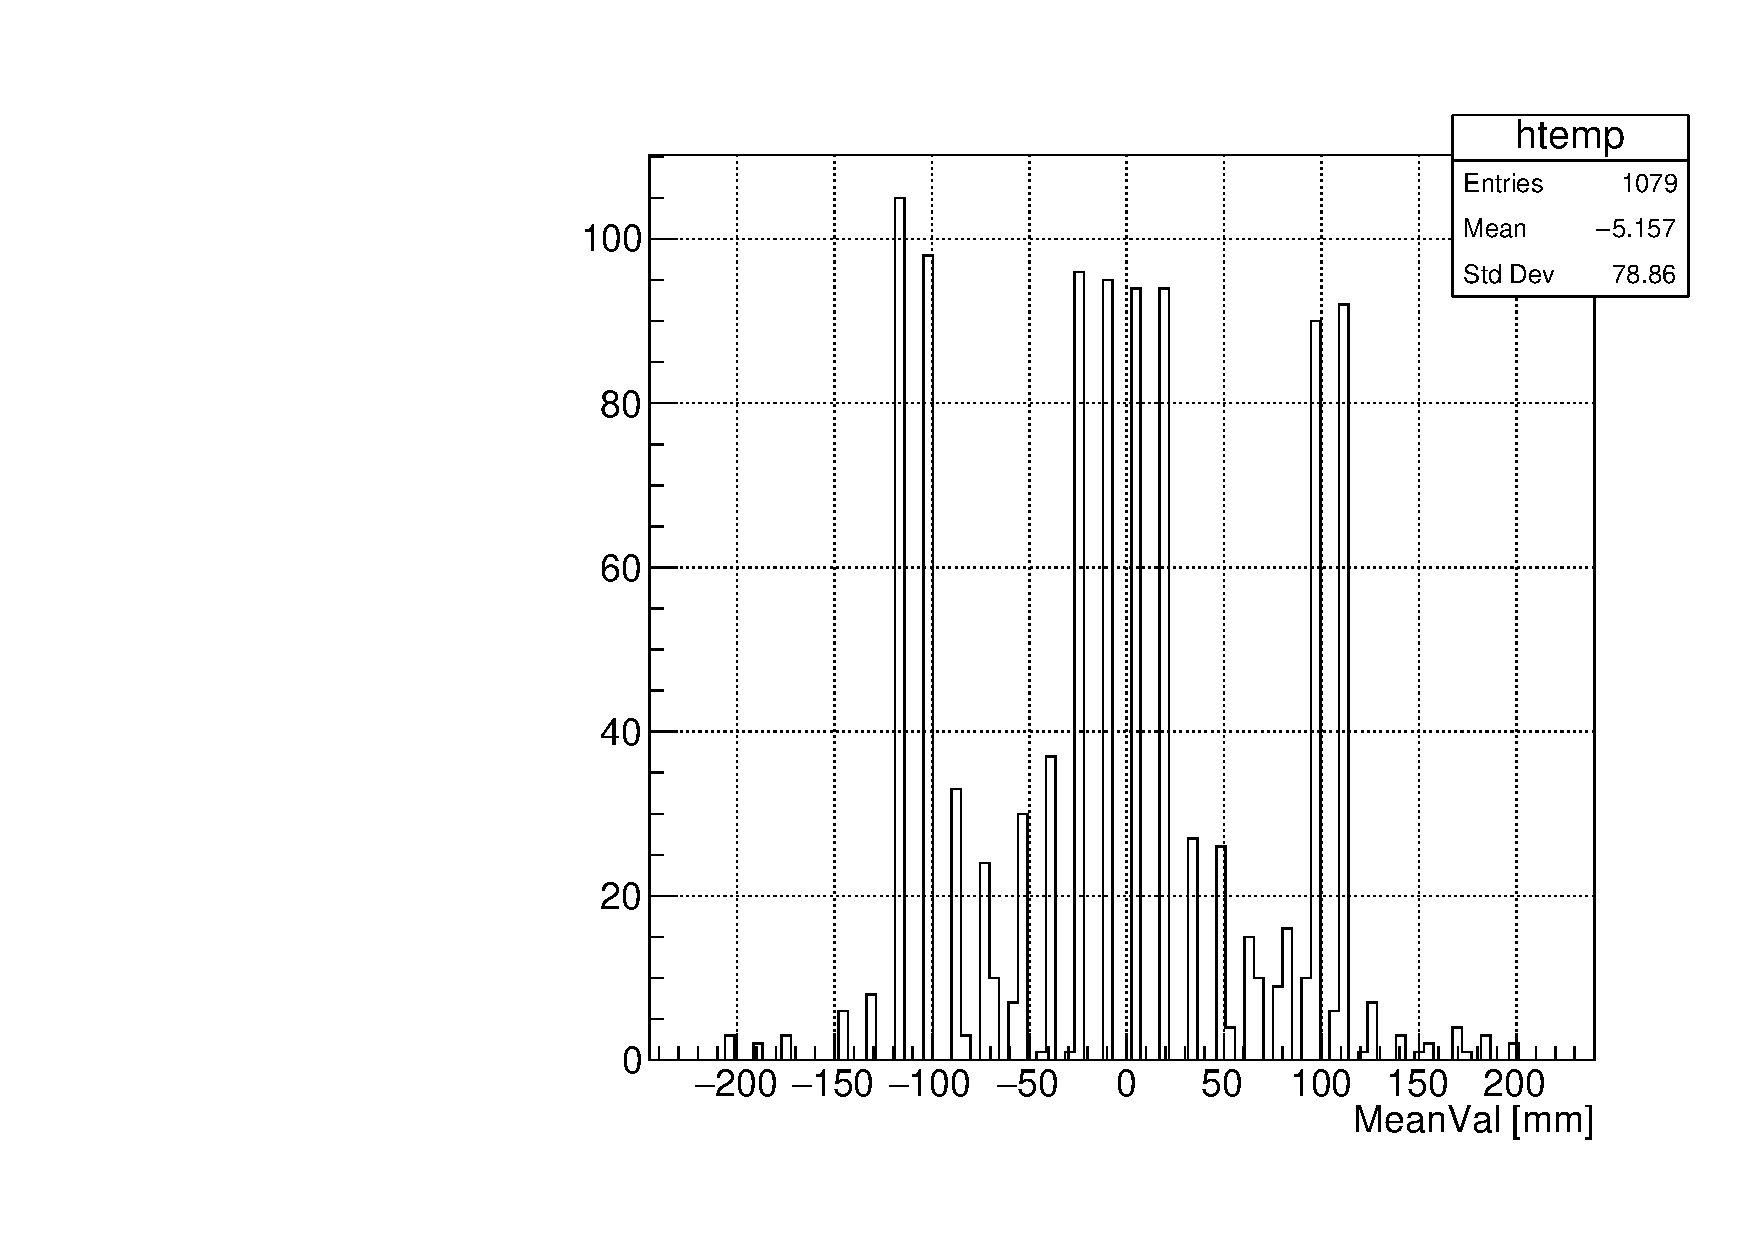
\includegraphics[width=.4\linewidth]{plots/2018/ZMeanVal.pdf}
    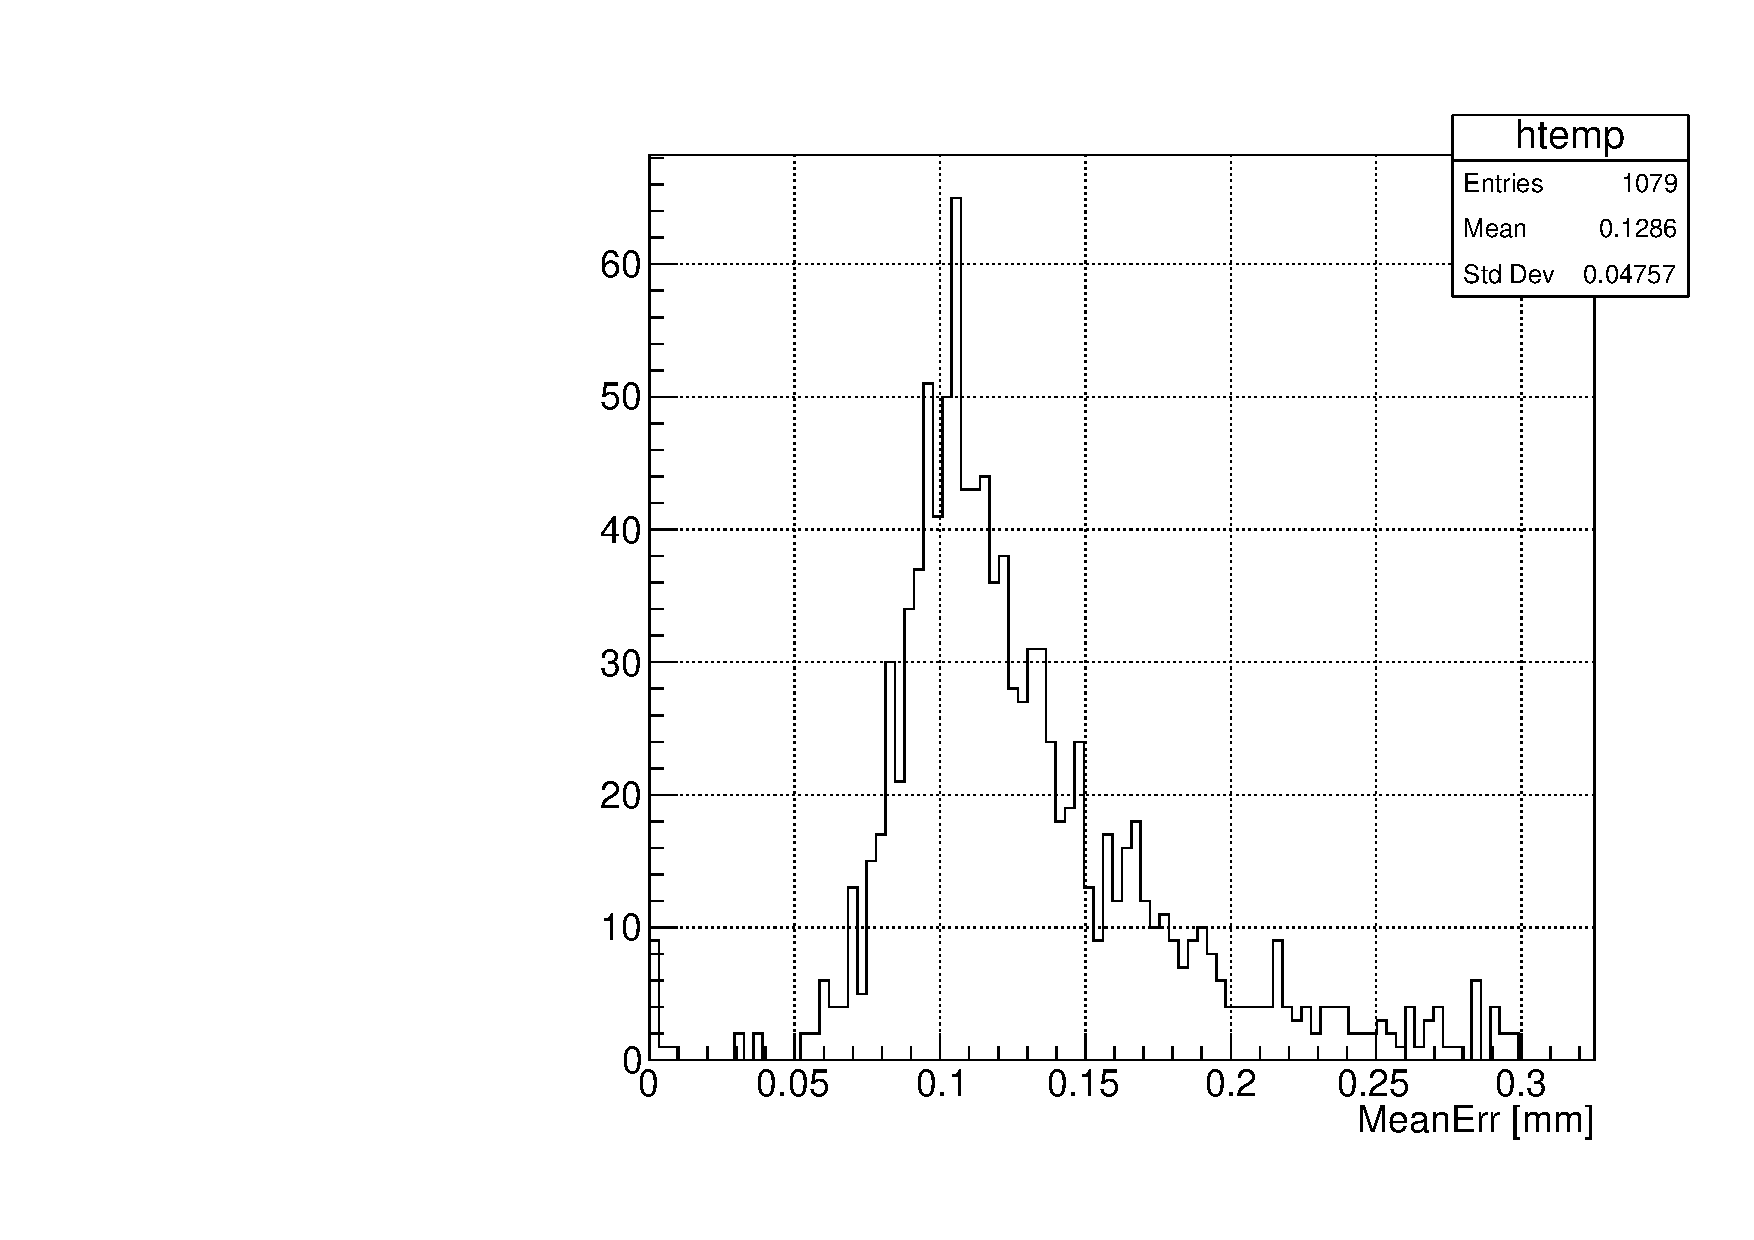
\includegraphics[width=.4\linewidth]{plots/2018/ZMeanErr.pdf}\\
    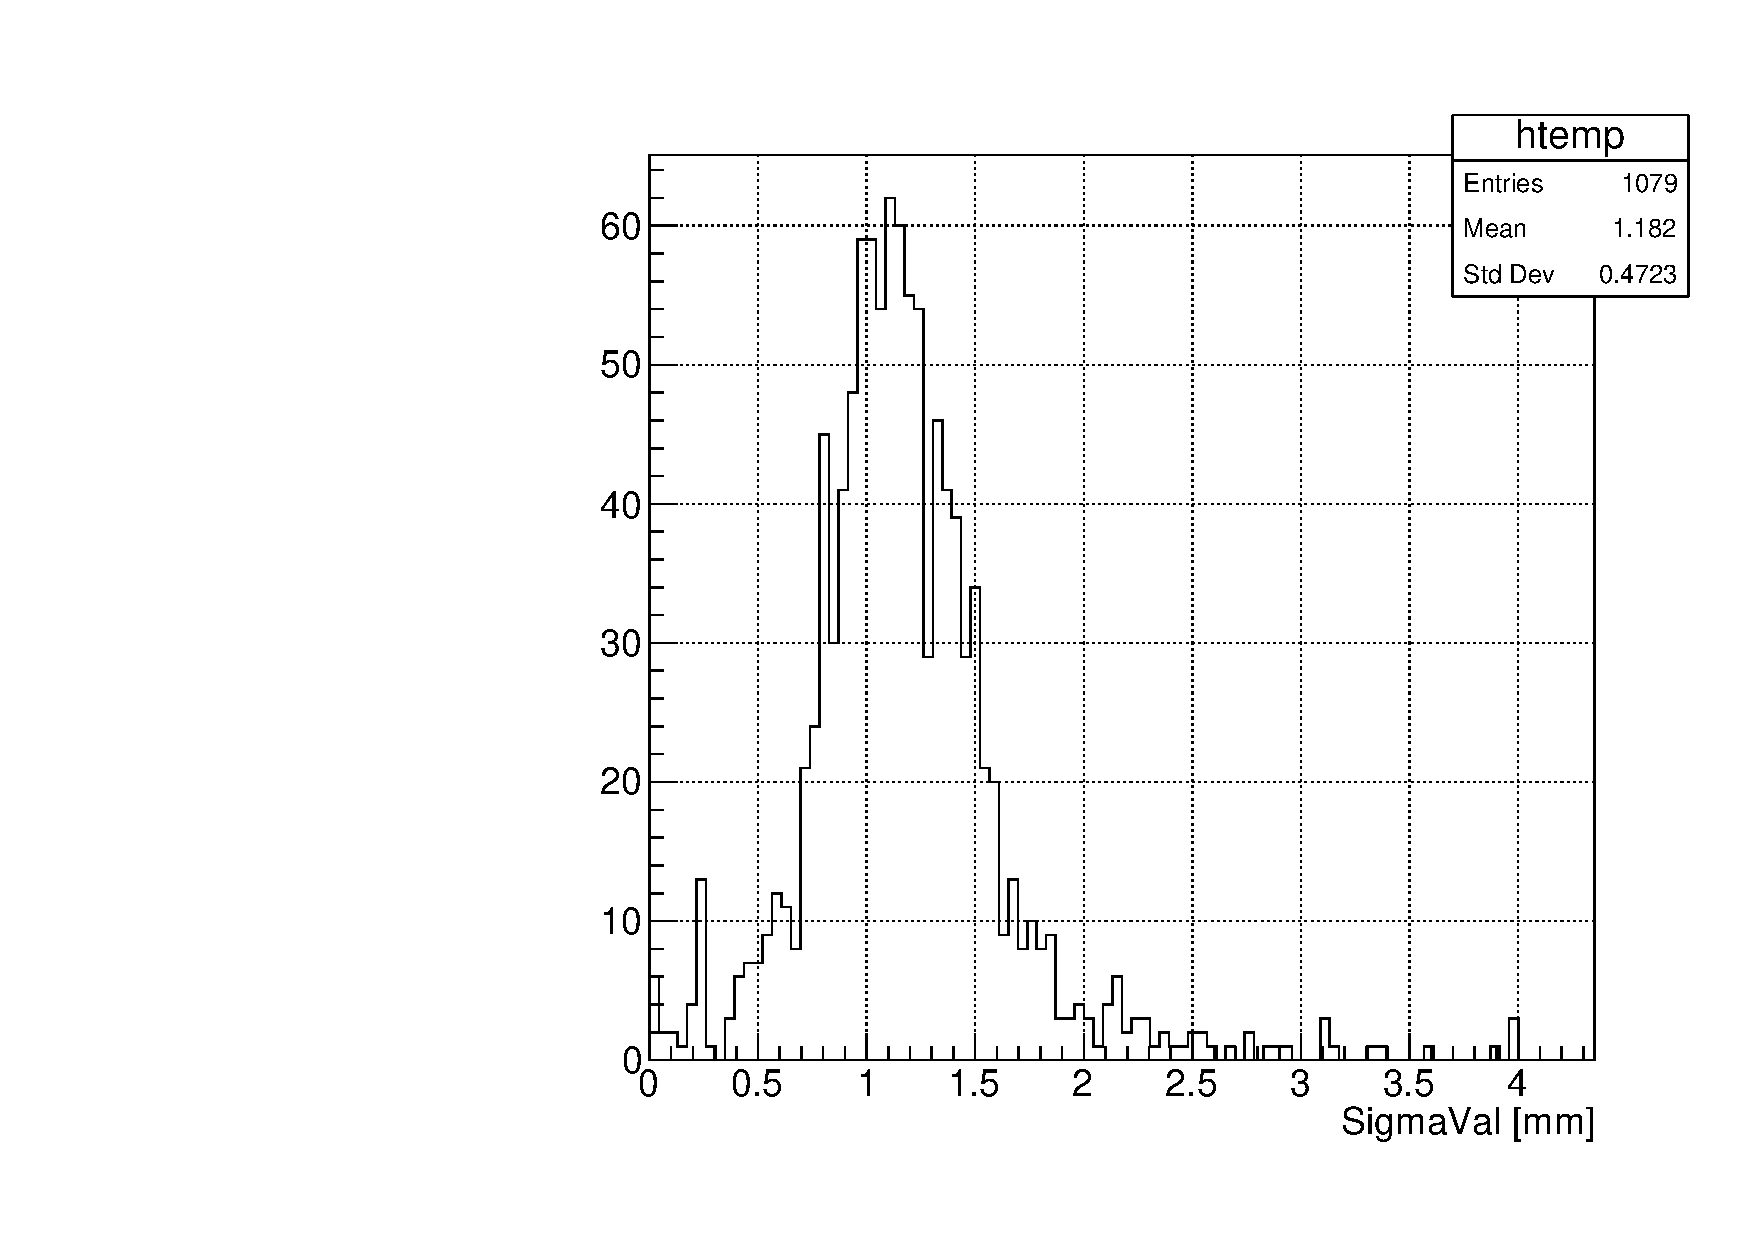
\includegraphics[width=.4\linewidth]{plots/2018/ZSigmaVal.pdf}
    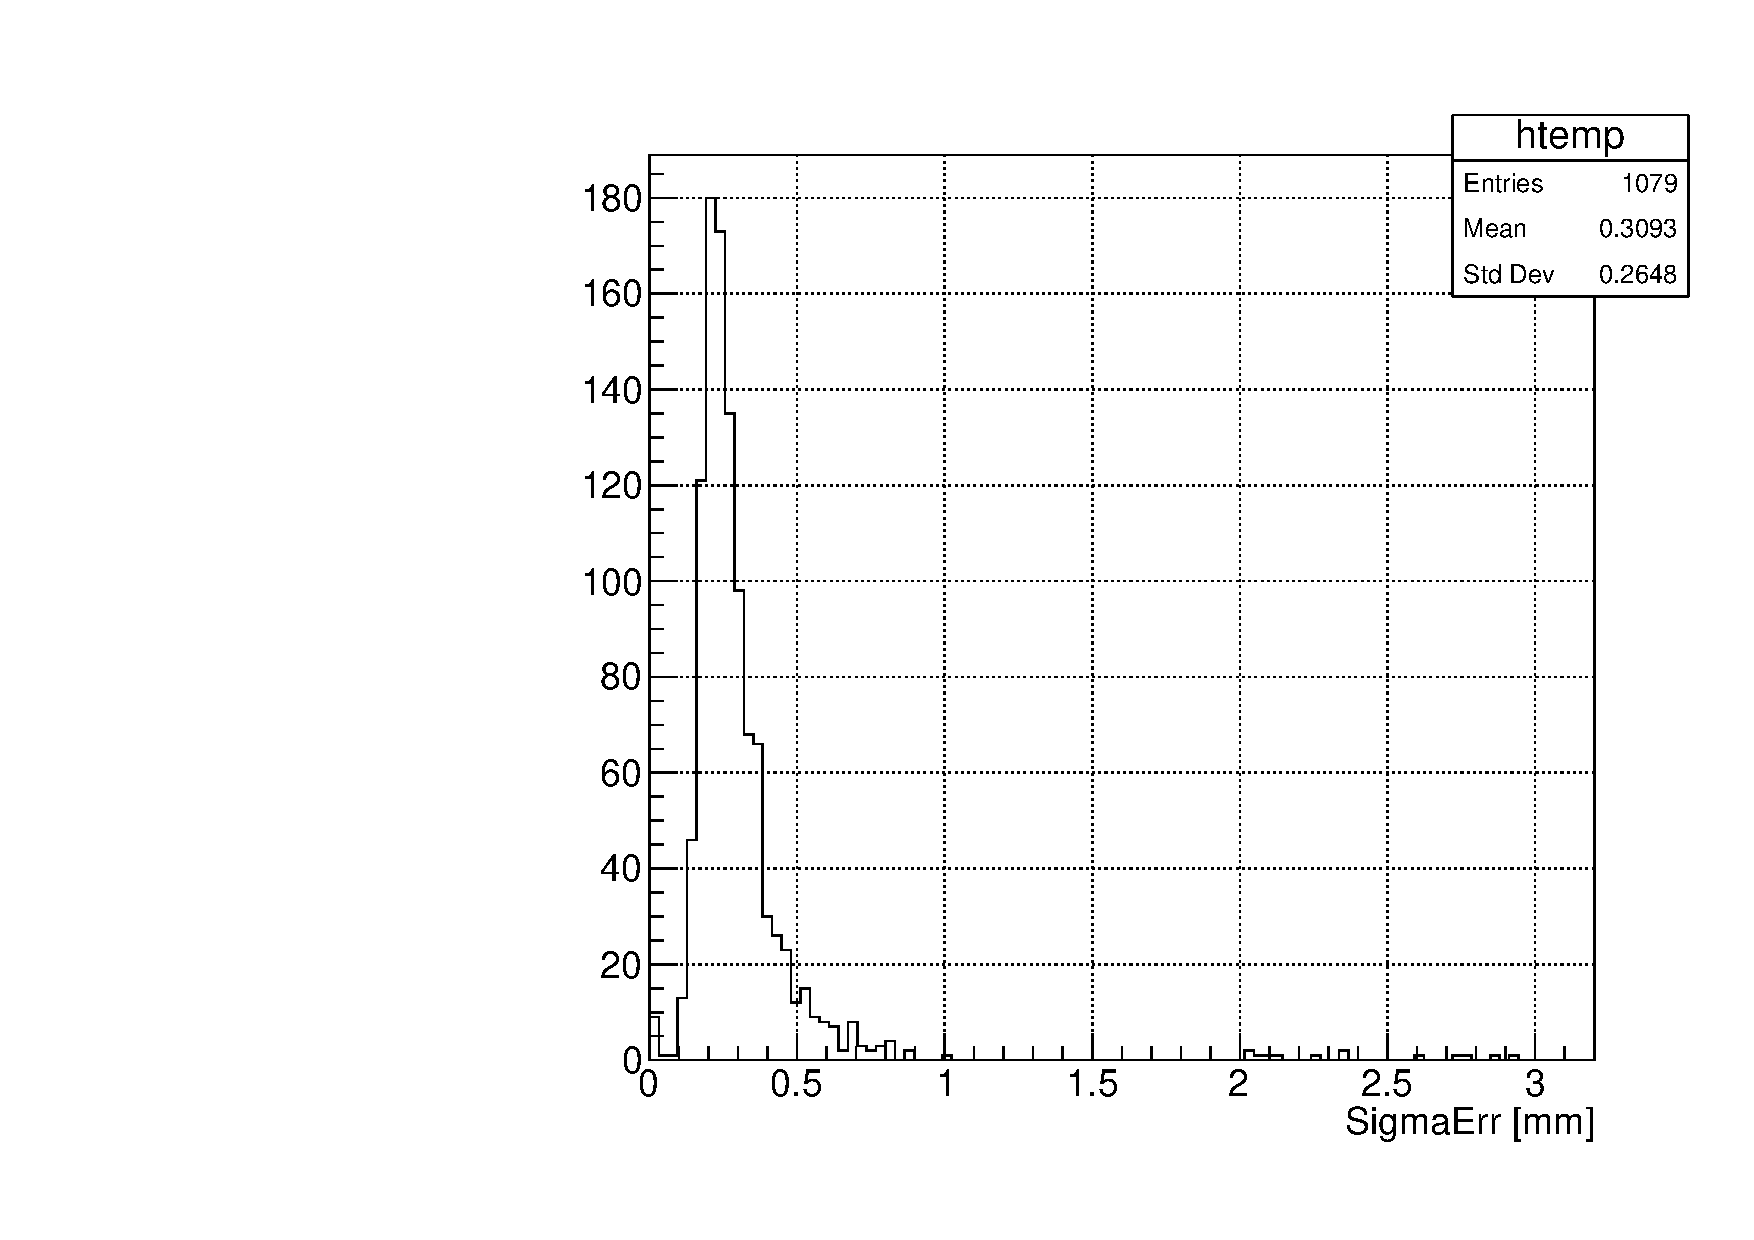
\includegraphics[width=.4\linewidth]{plots/2018/ZSigmaErr.pdf}\\
    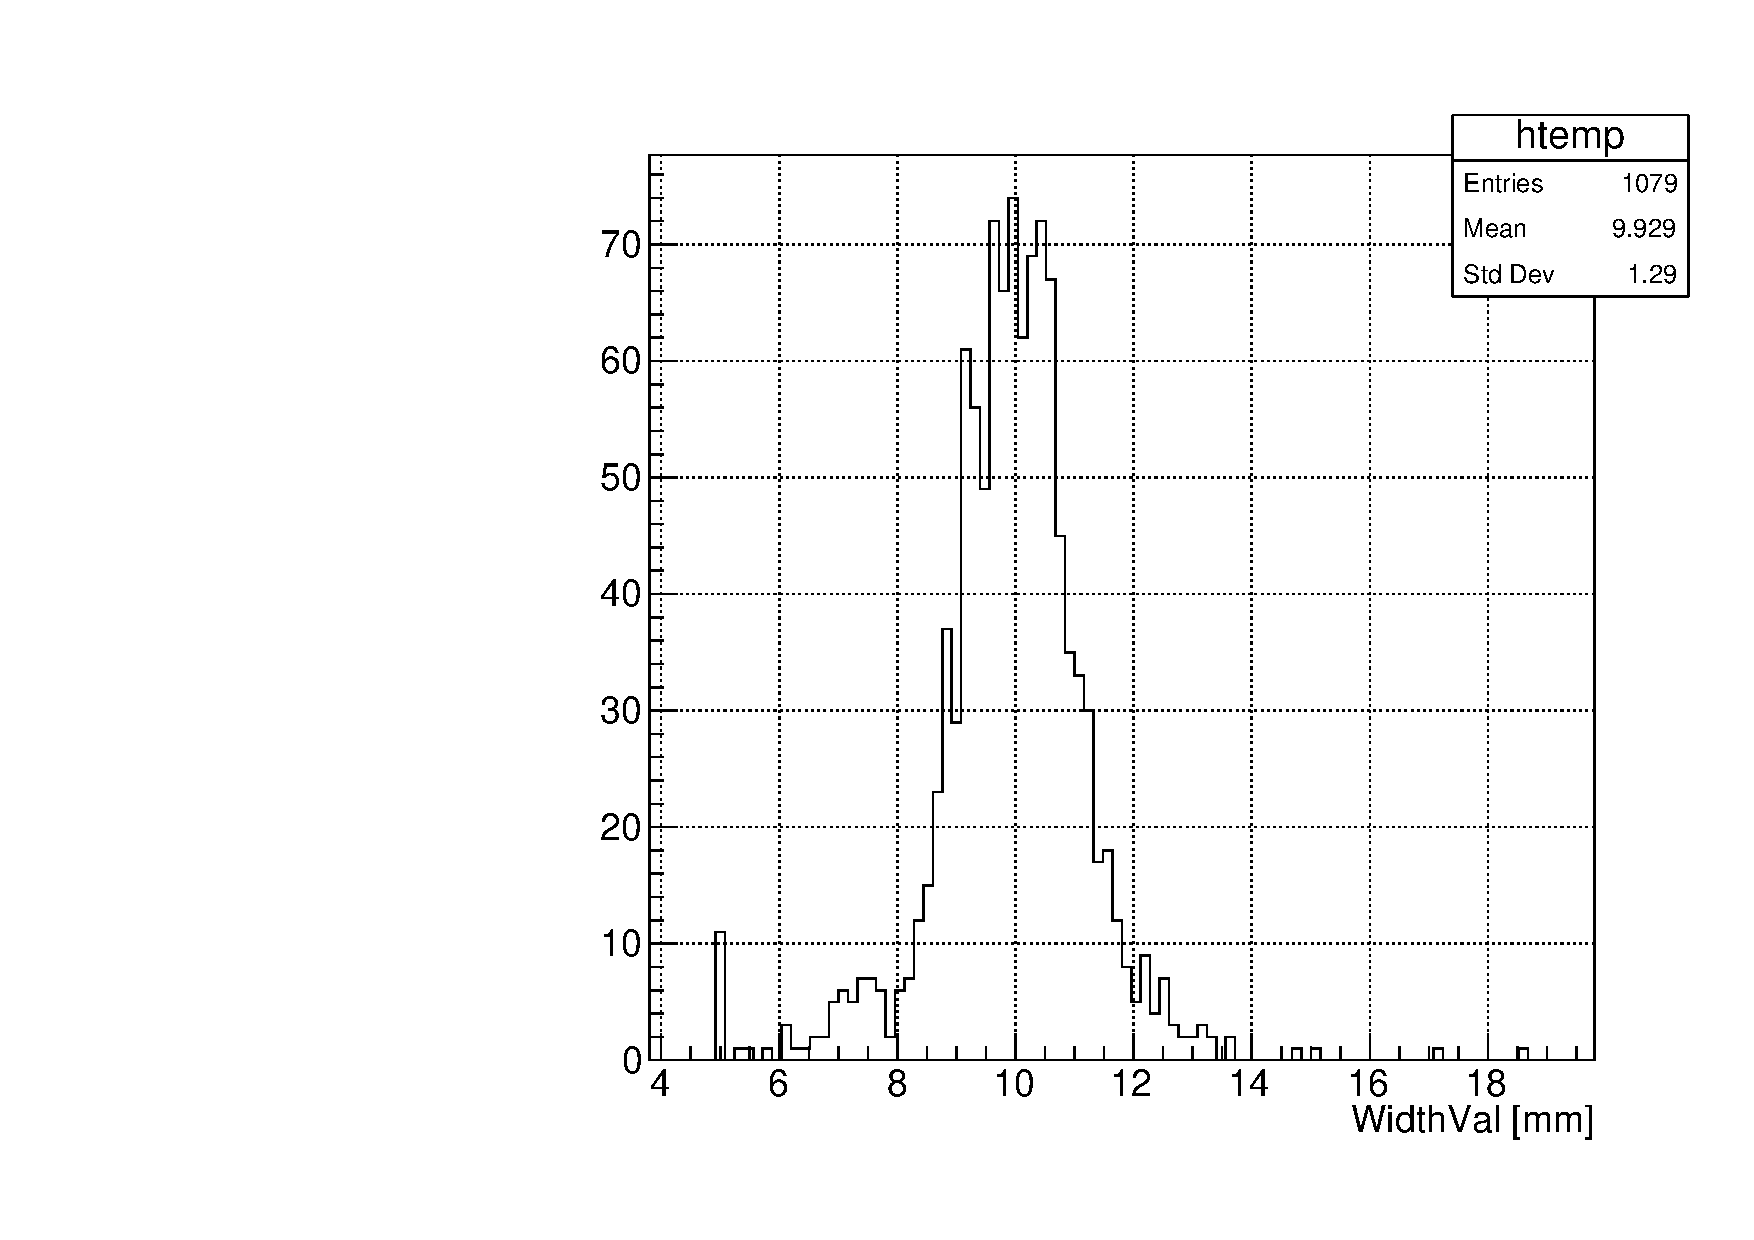
\includegraphics[width=.4\linewidth]{plots/2018/ZWidthVal.pdf}
    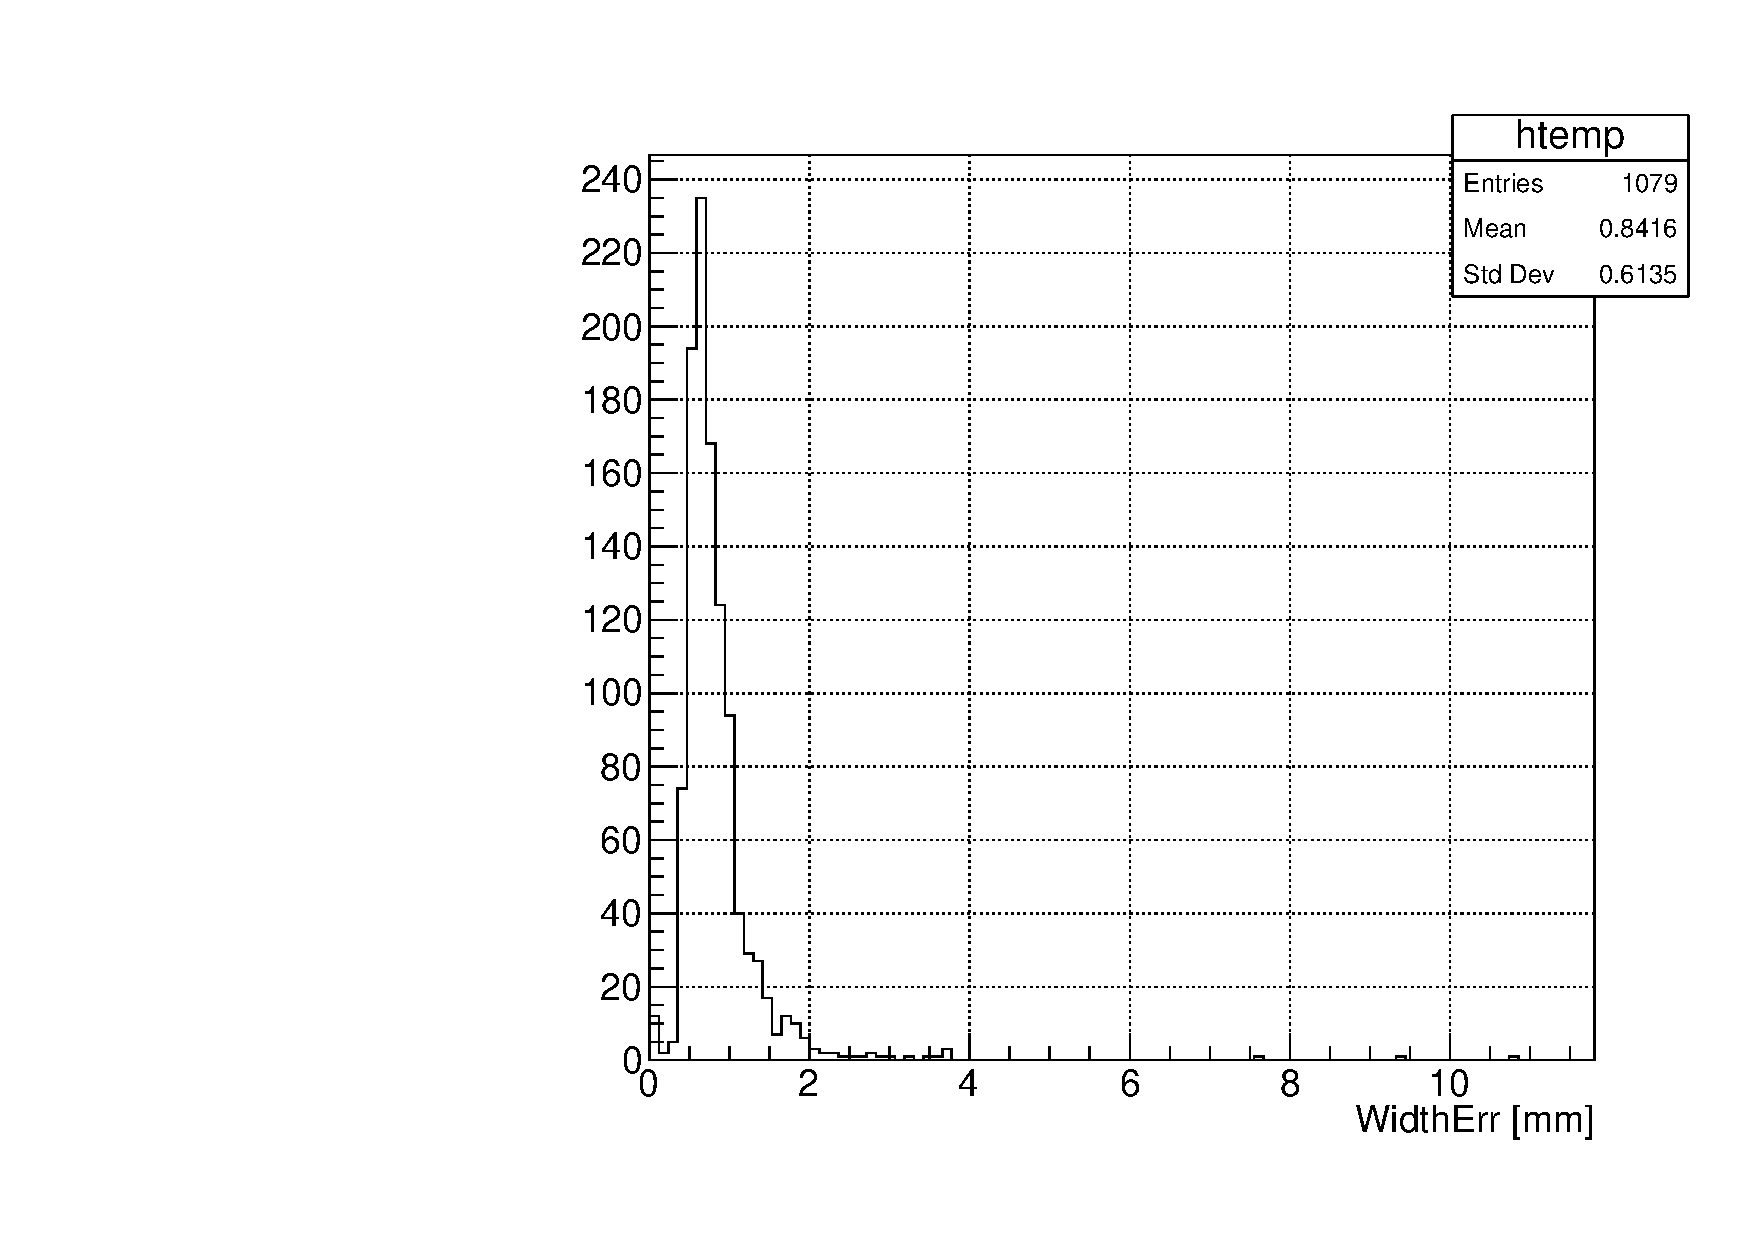
\includegraphics[width=.4\linewidth]{plots/2018/ZWidthErr.pdf}\\
    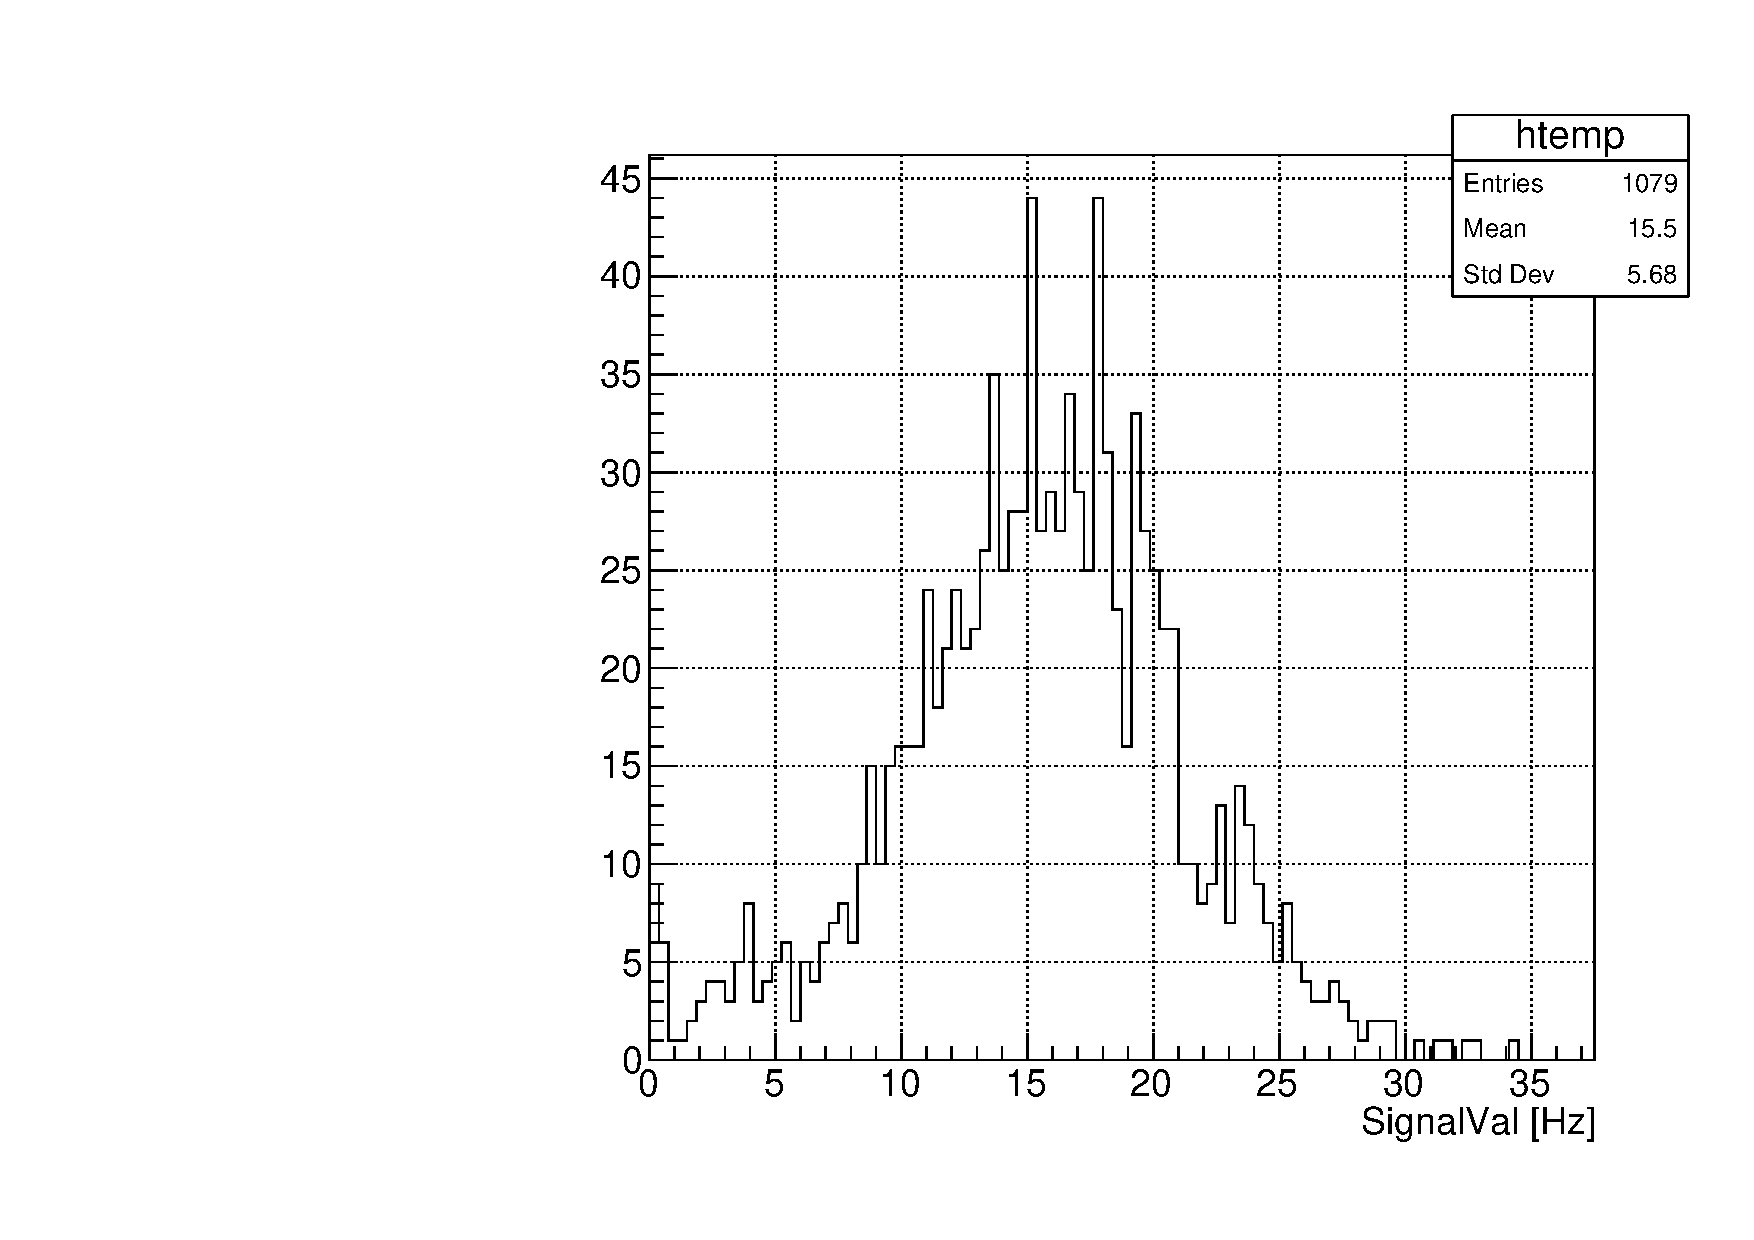
\includegraphics[width=.4\linewidth]{plots/2018/ZSignalVal.pdf}
    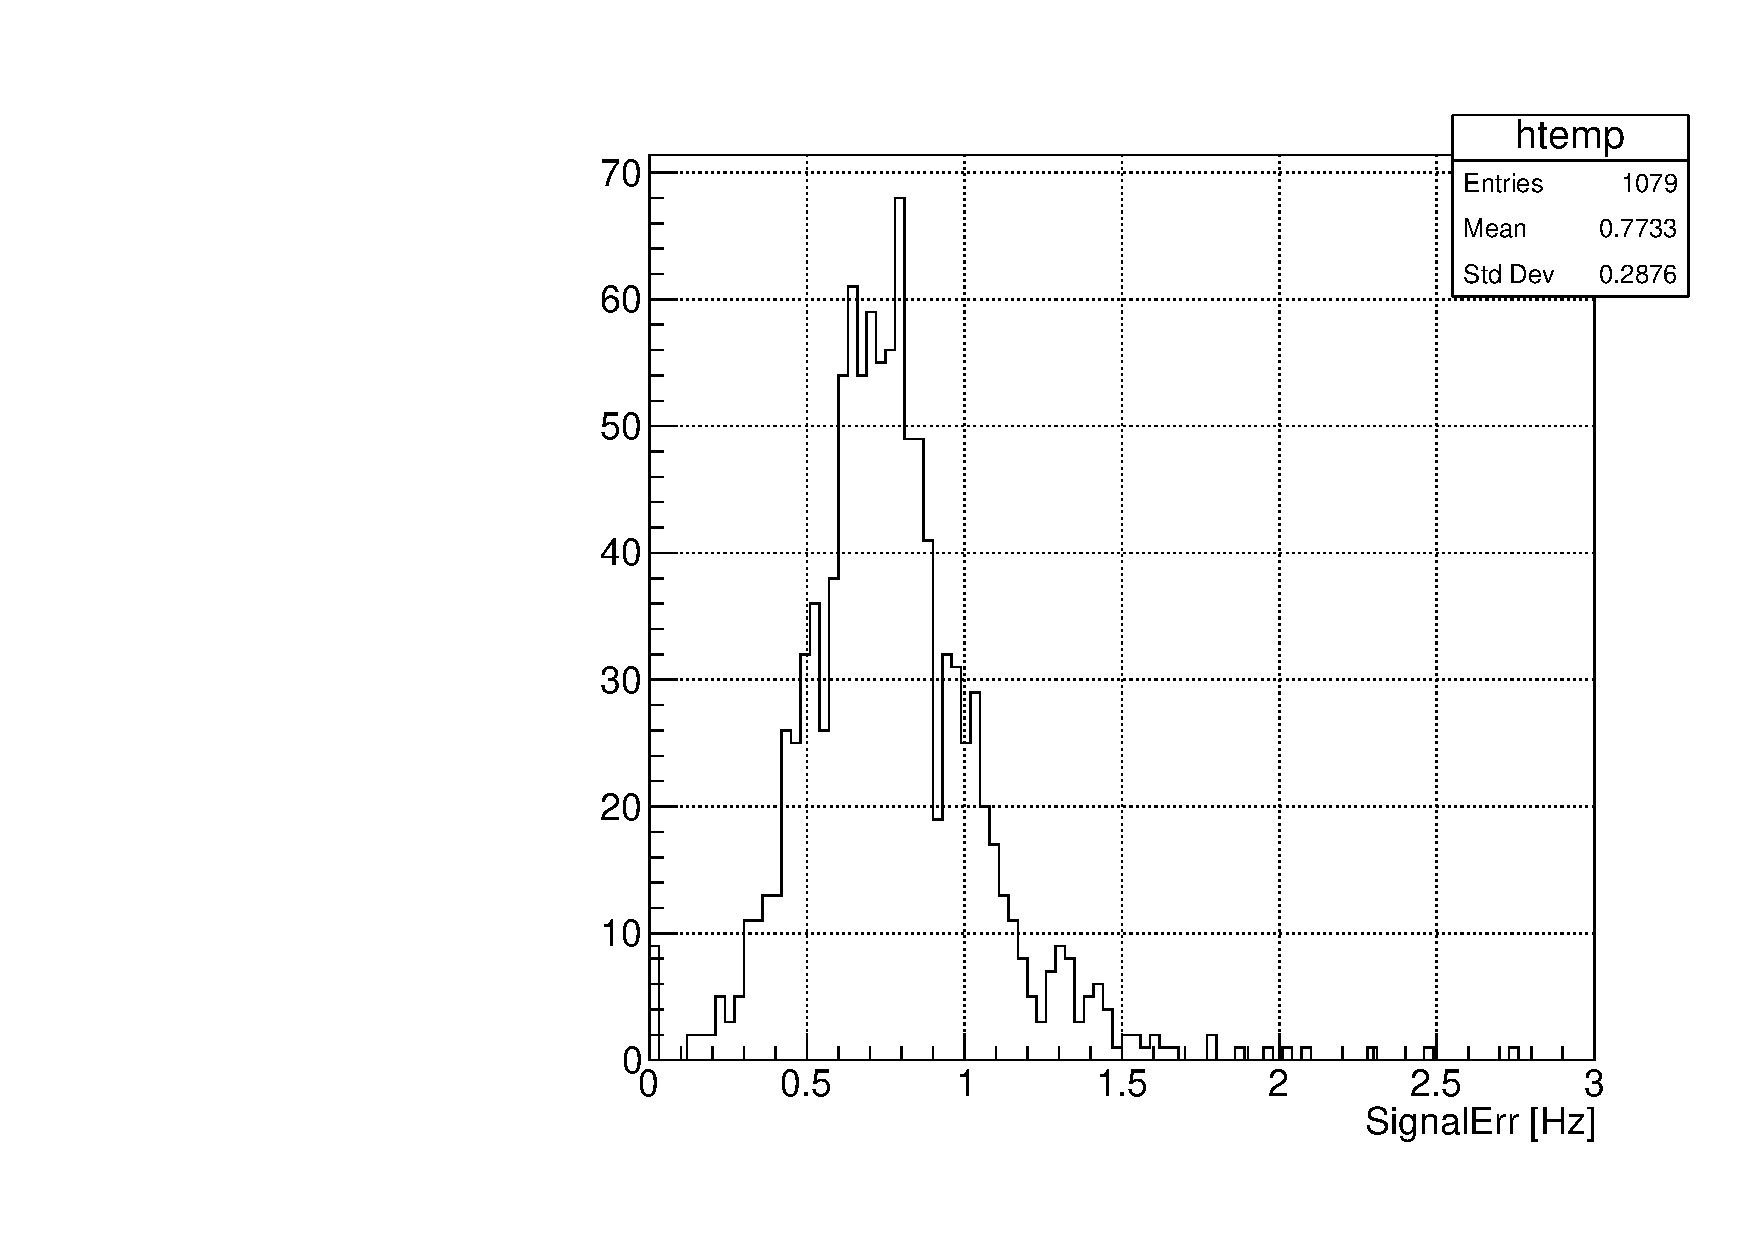
\includegraphics[width=.4\linewidth]{plots/2018/ZSignalErr.pdf}\\
    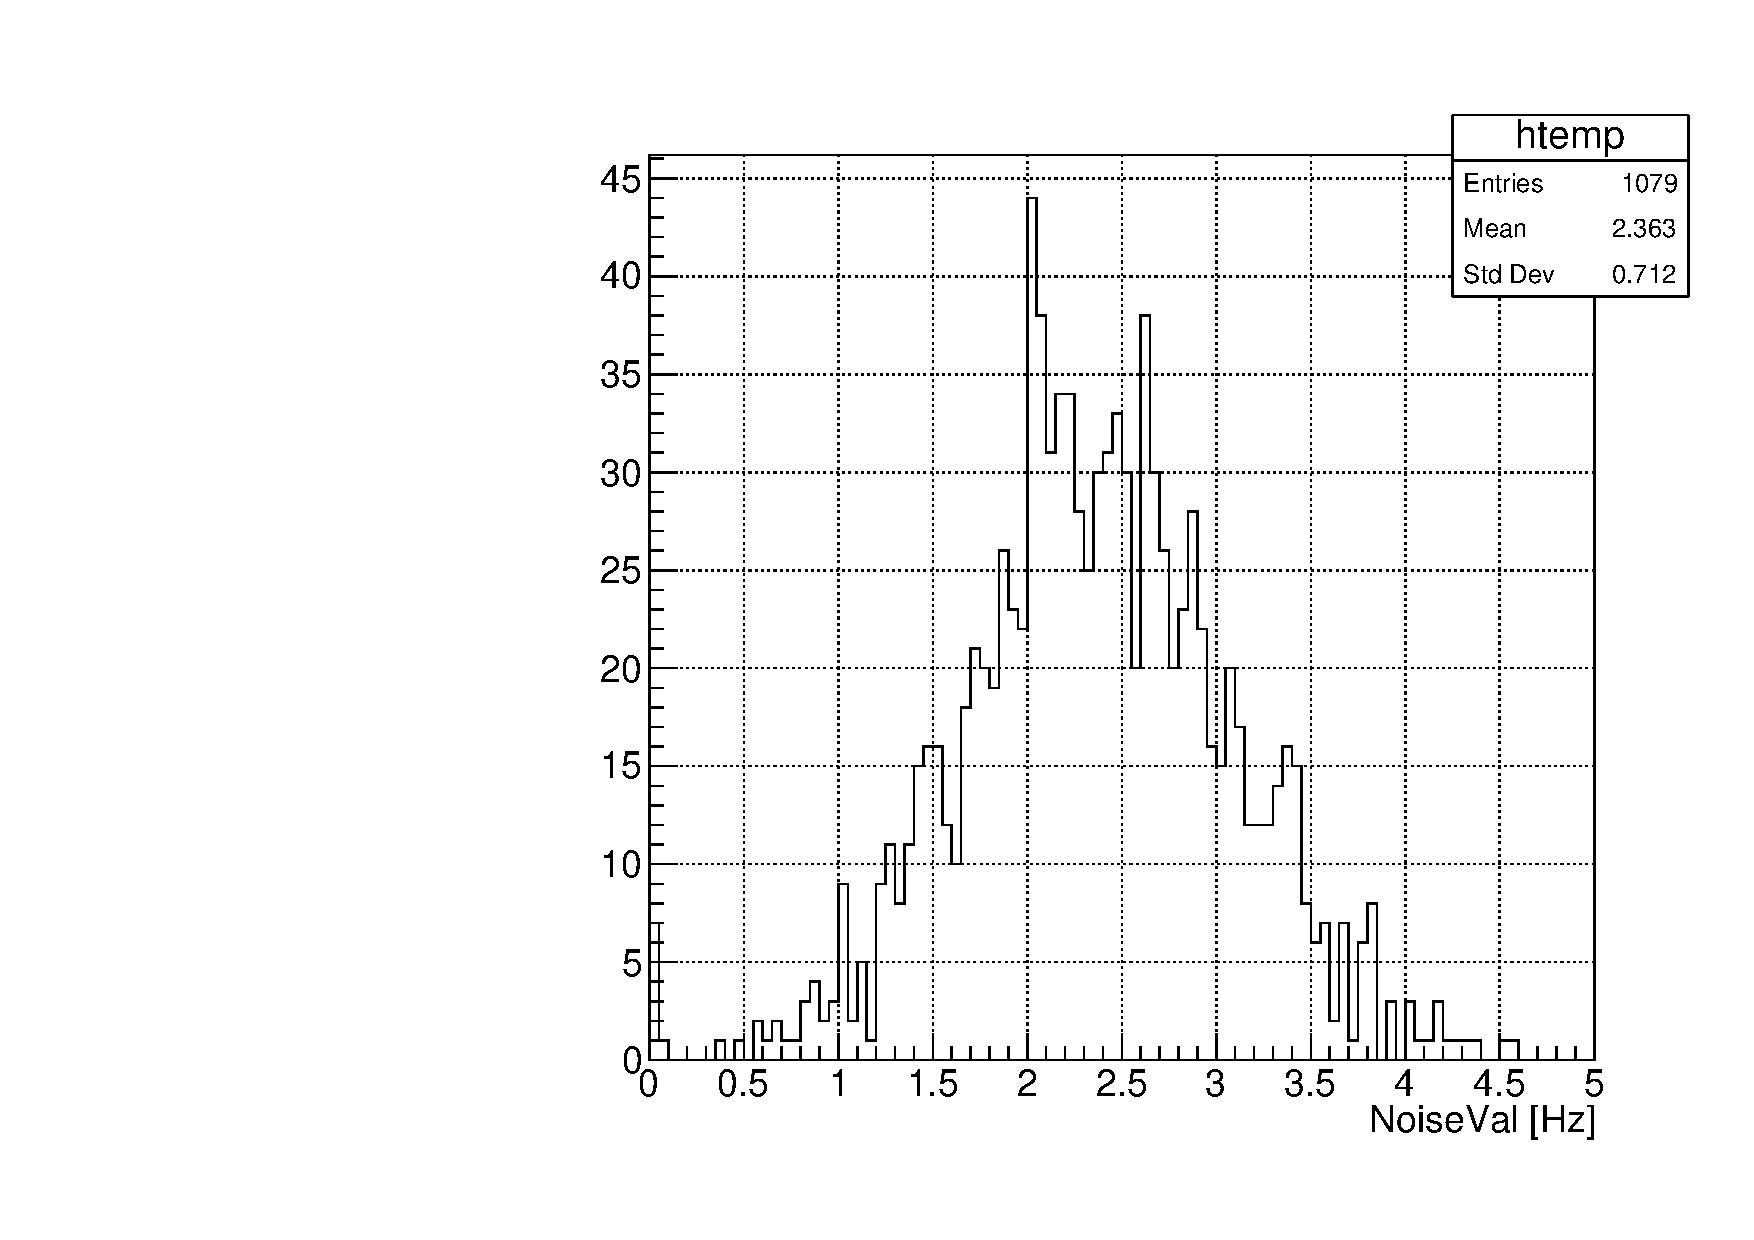
\includegraphics[width=.4\linewidth]{plots/2018/ZNoiseVal.pdf}
    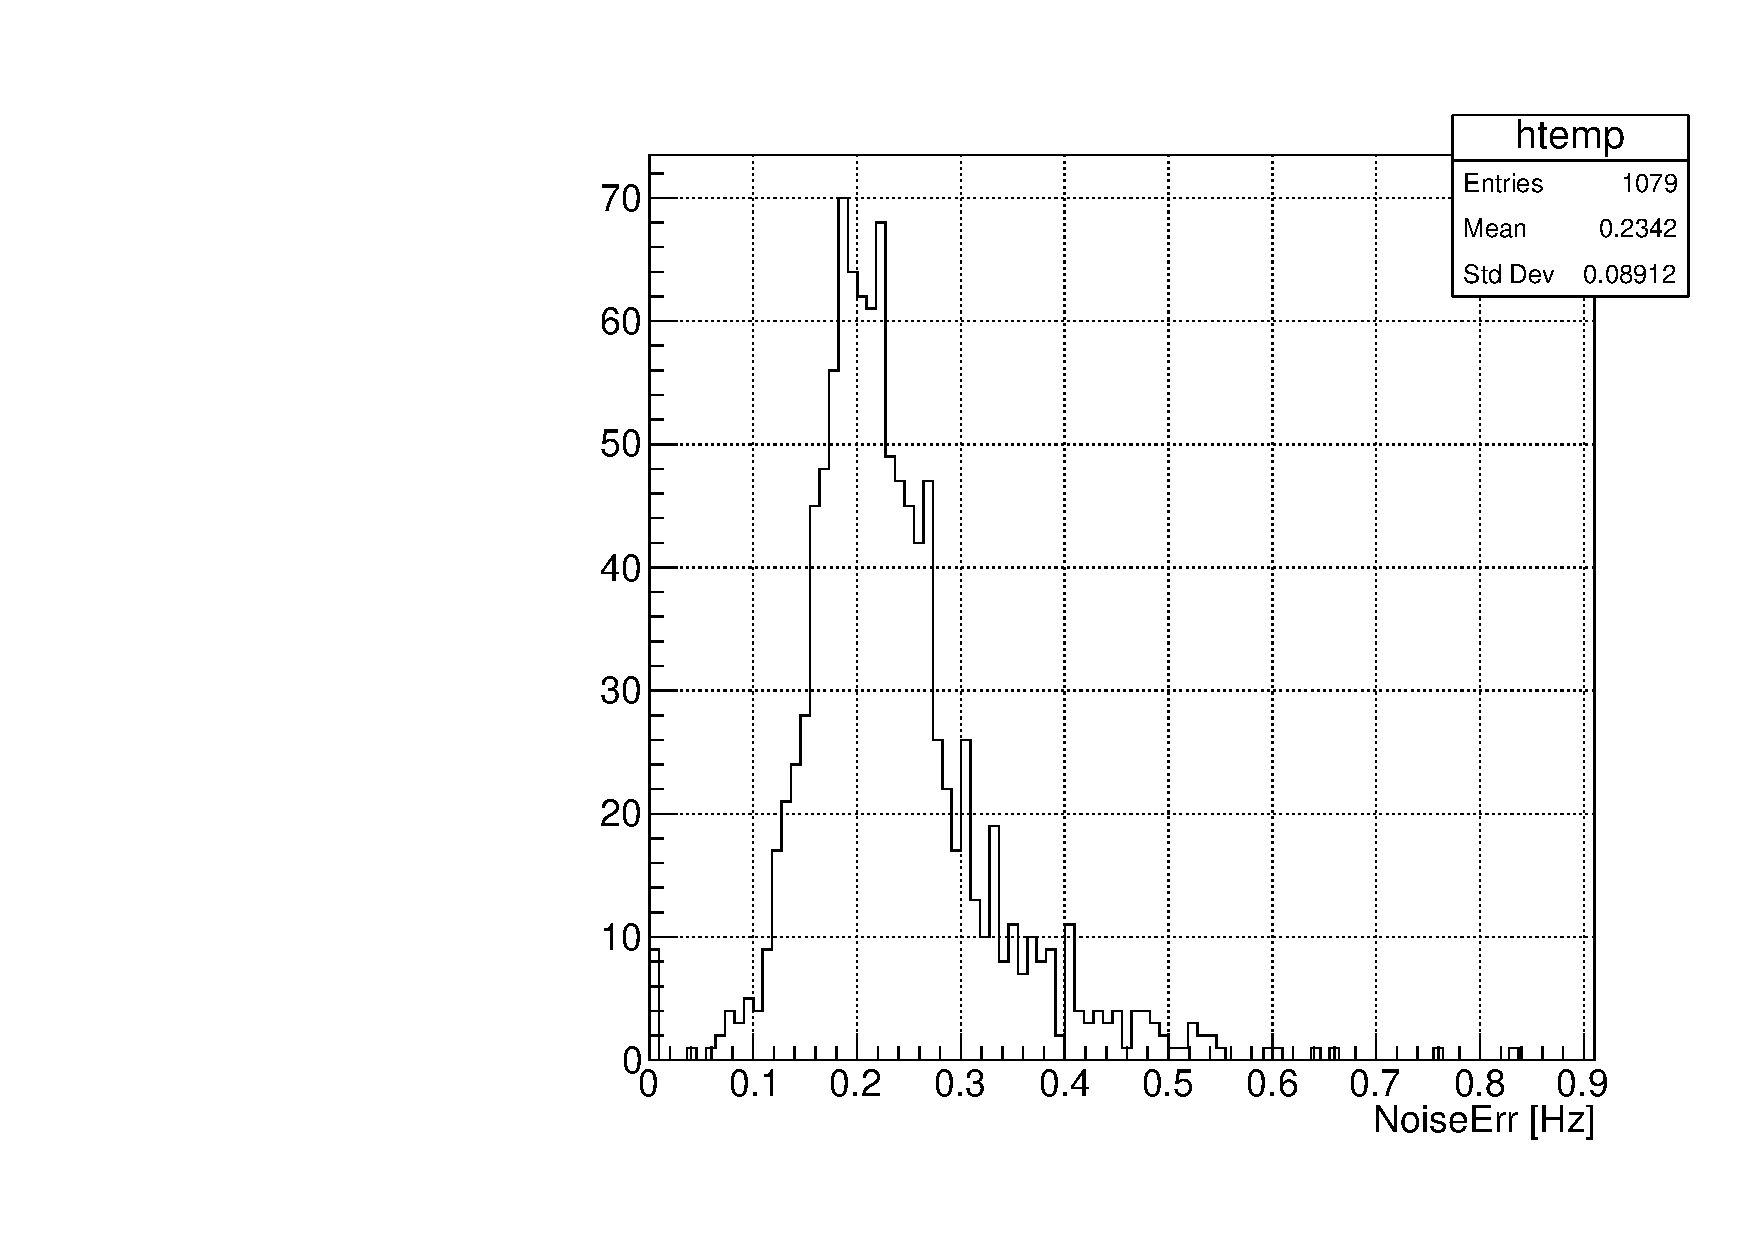
\includegraphics[width=.4\linewidth]{plots/2018/ZNoiseErr.pdf}
    \caption{Fitted parameter values (left) and errors (right) for Z position fits.}
    \label{fig:zfitpars}
\end{figure}

\begin{figure}[h]
    \centering
    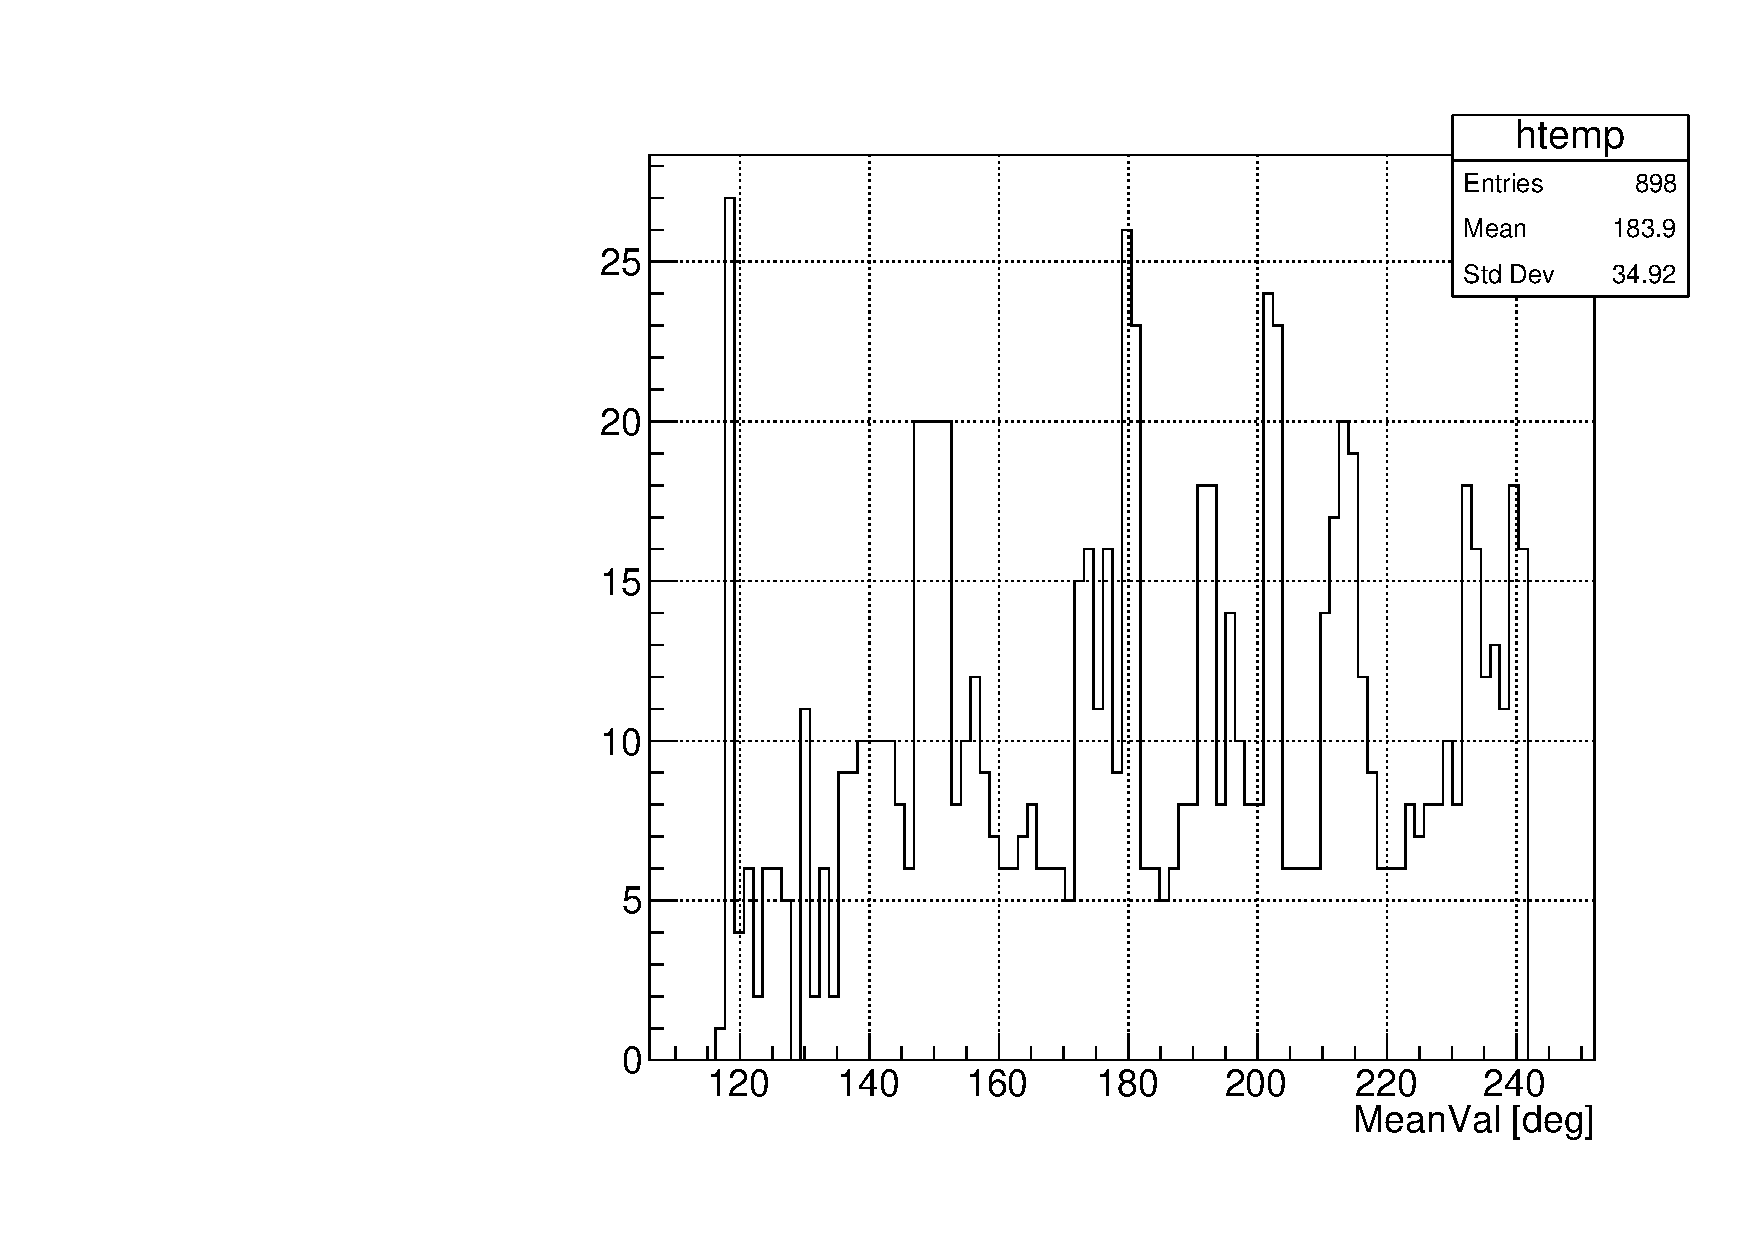
\includegraphics[width=.4\linewidth]{plots/2018/PhiMeanVal.pdf}
    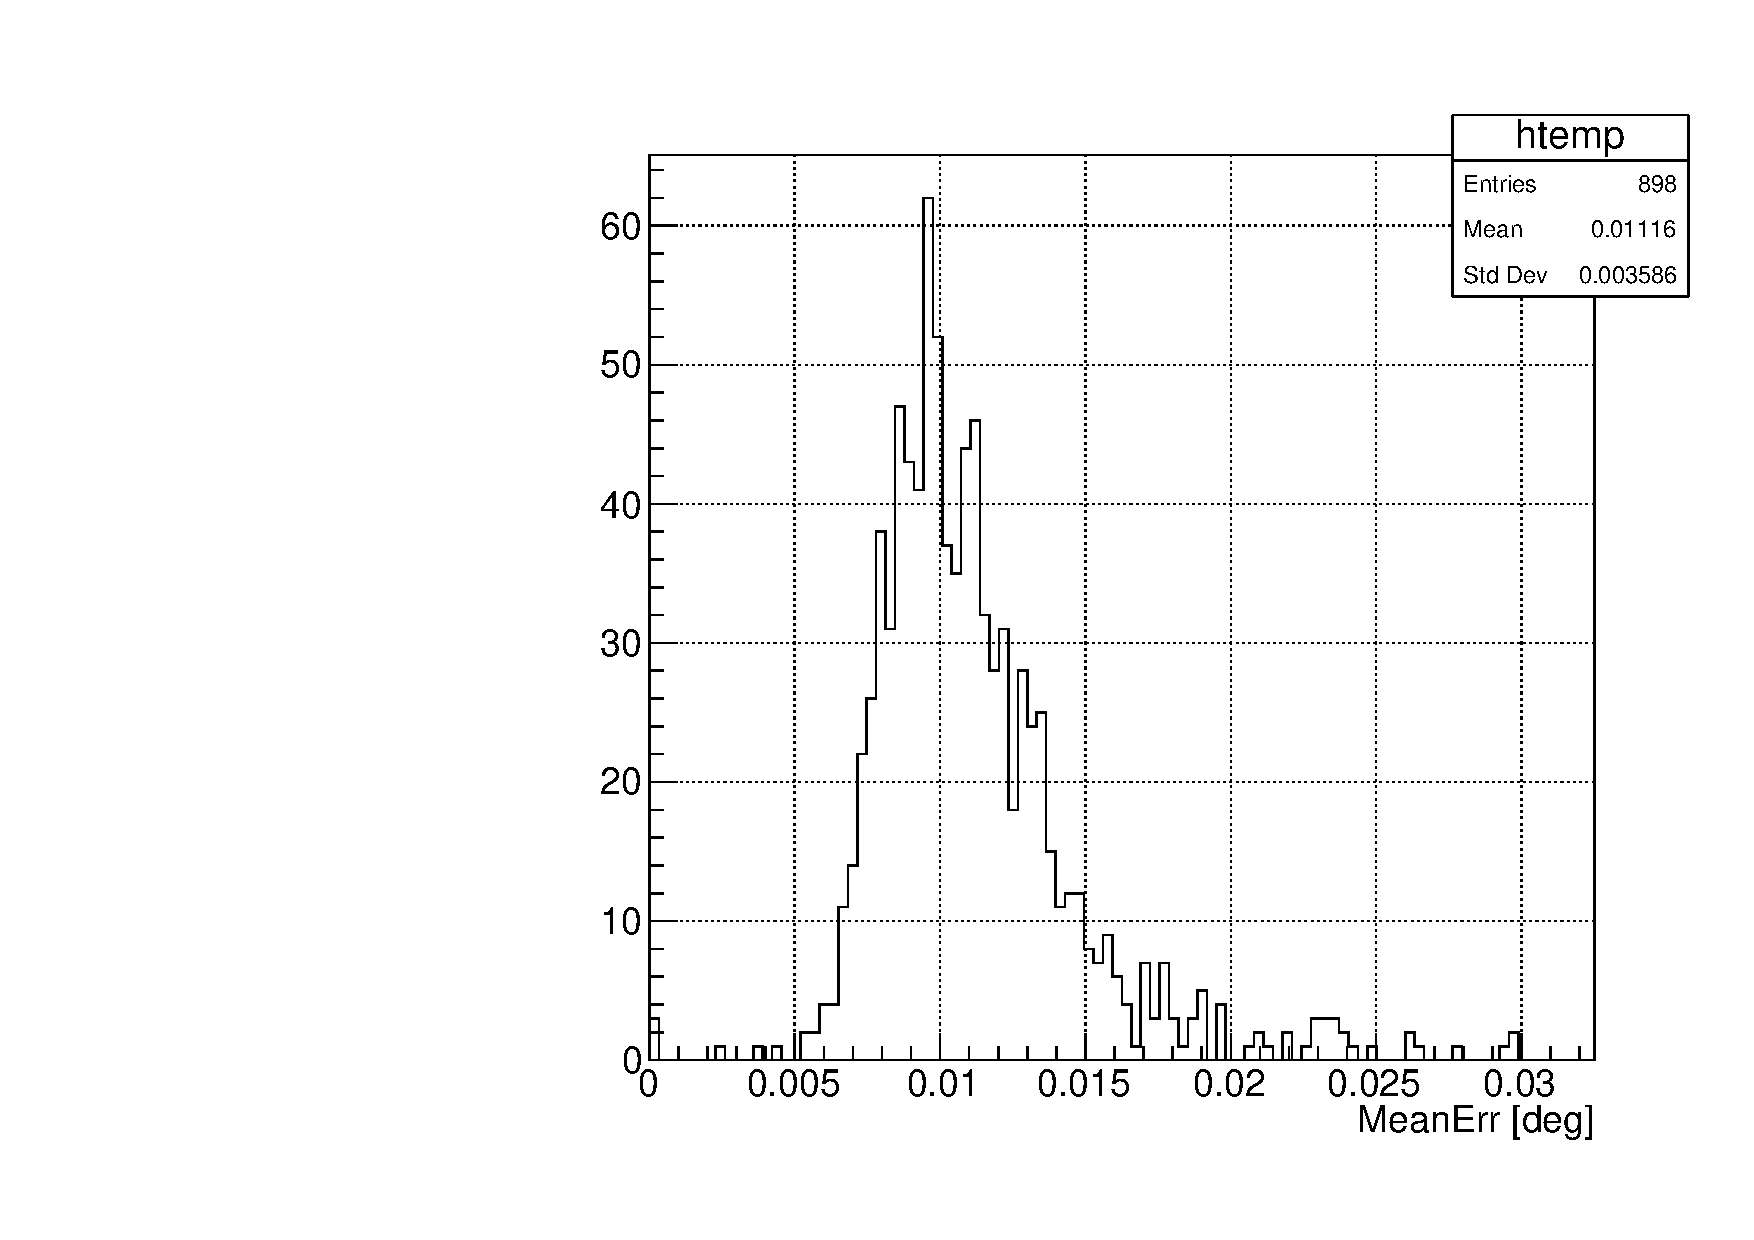
\includegraphics[width=.4\linewidth]{plots/2018/PhiMeanErr.pdf}\\
    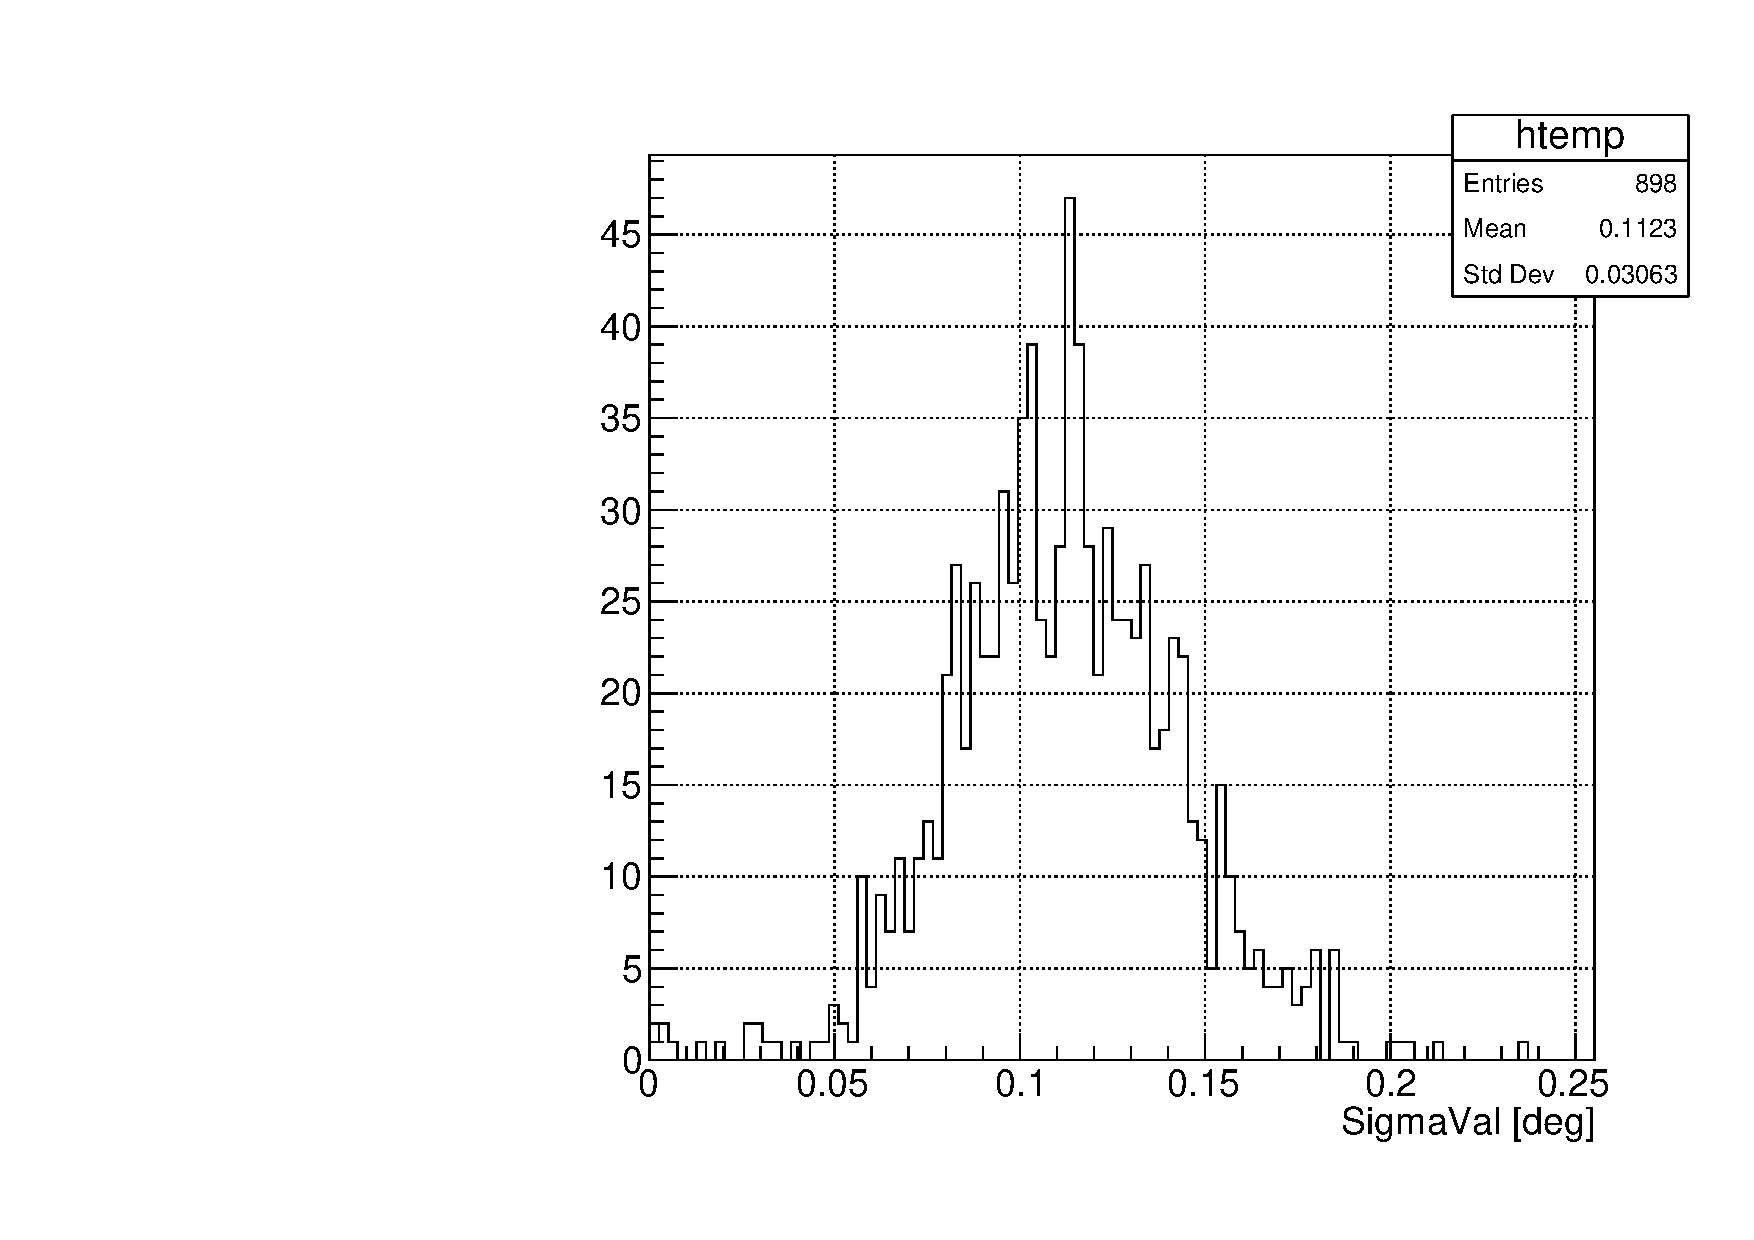
\includegraphics[width=.4\linewidth]{plots/2018/PhiSigmaVal.pdf}
    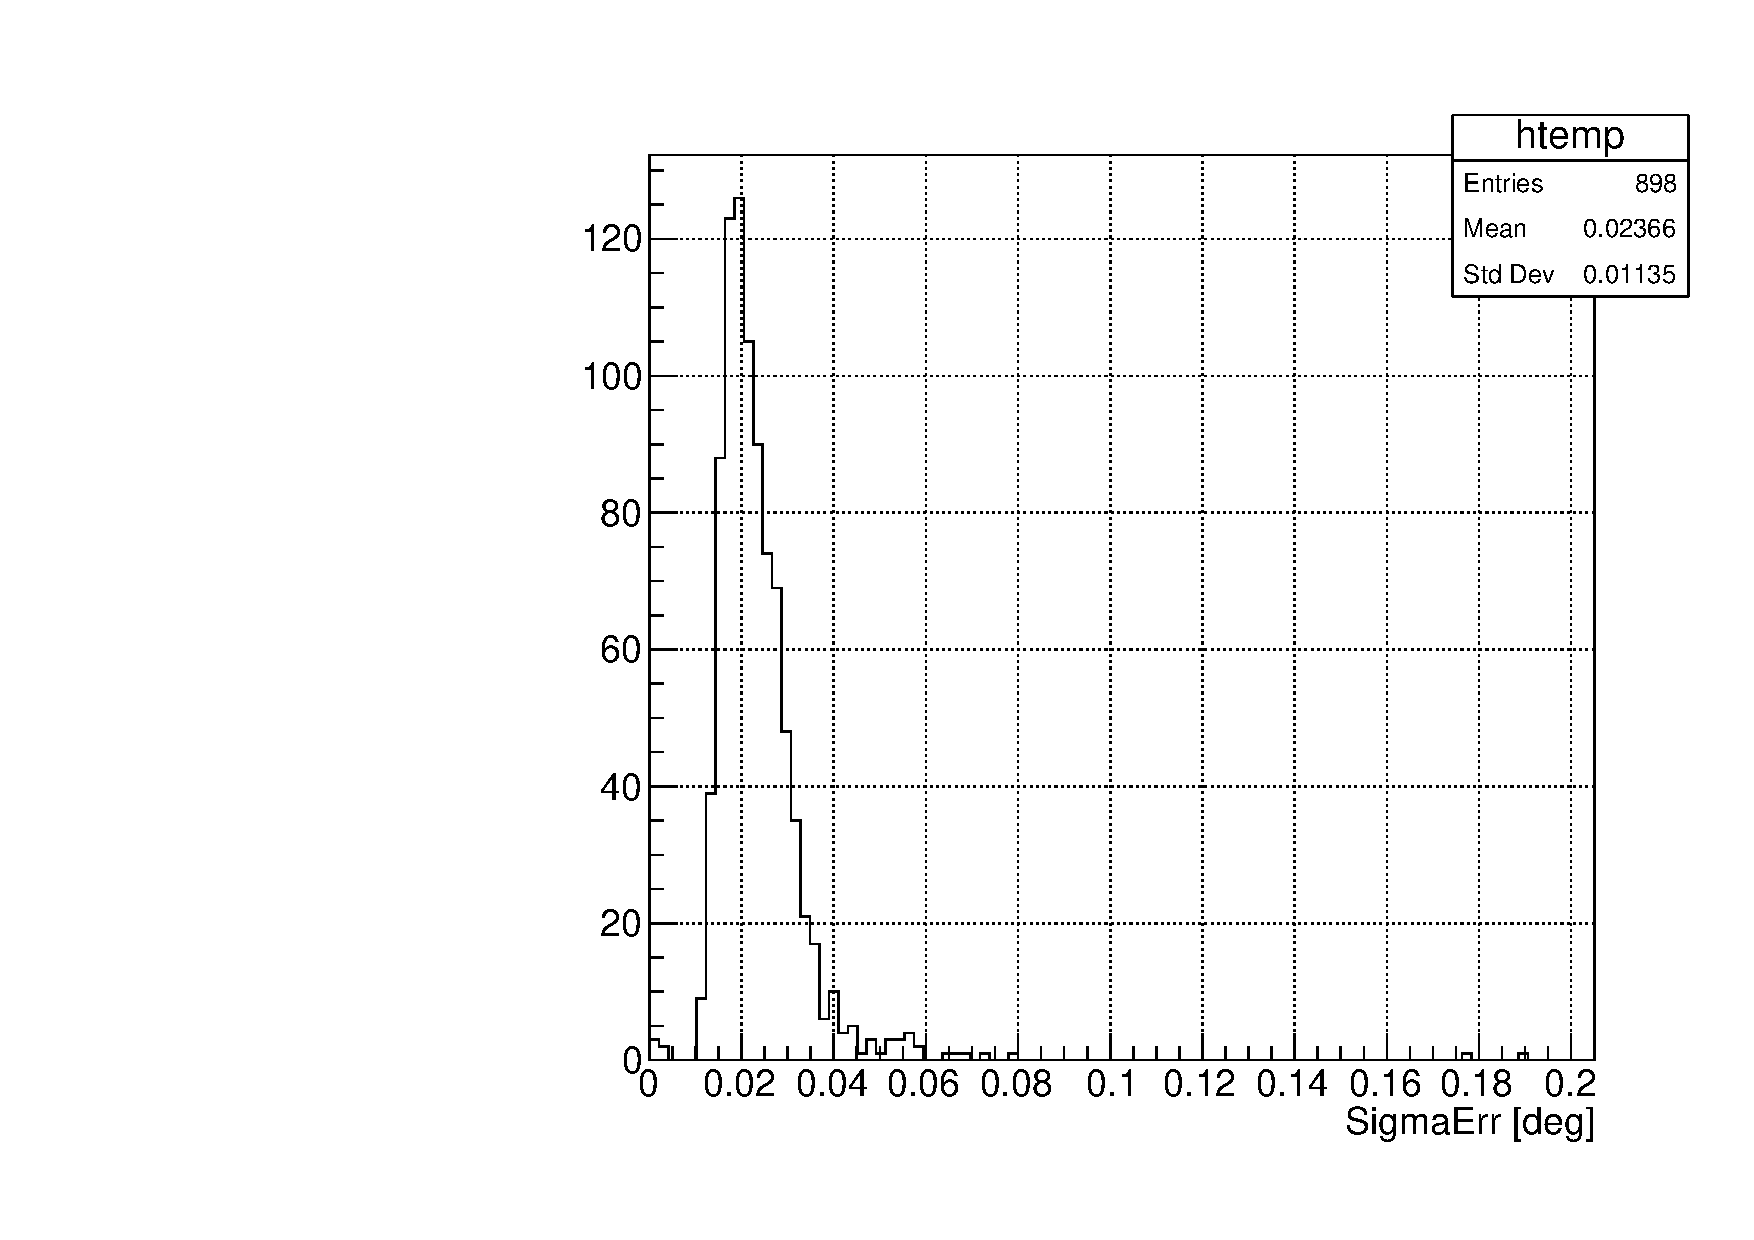
\includegraphics[width=.4\linewidth]{plots/2018/PhiSigmaErr.pdf}\\
    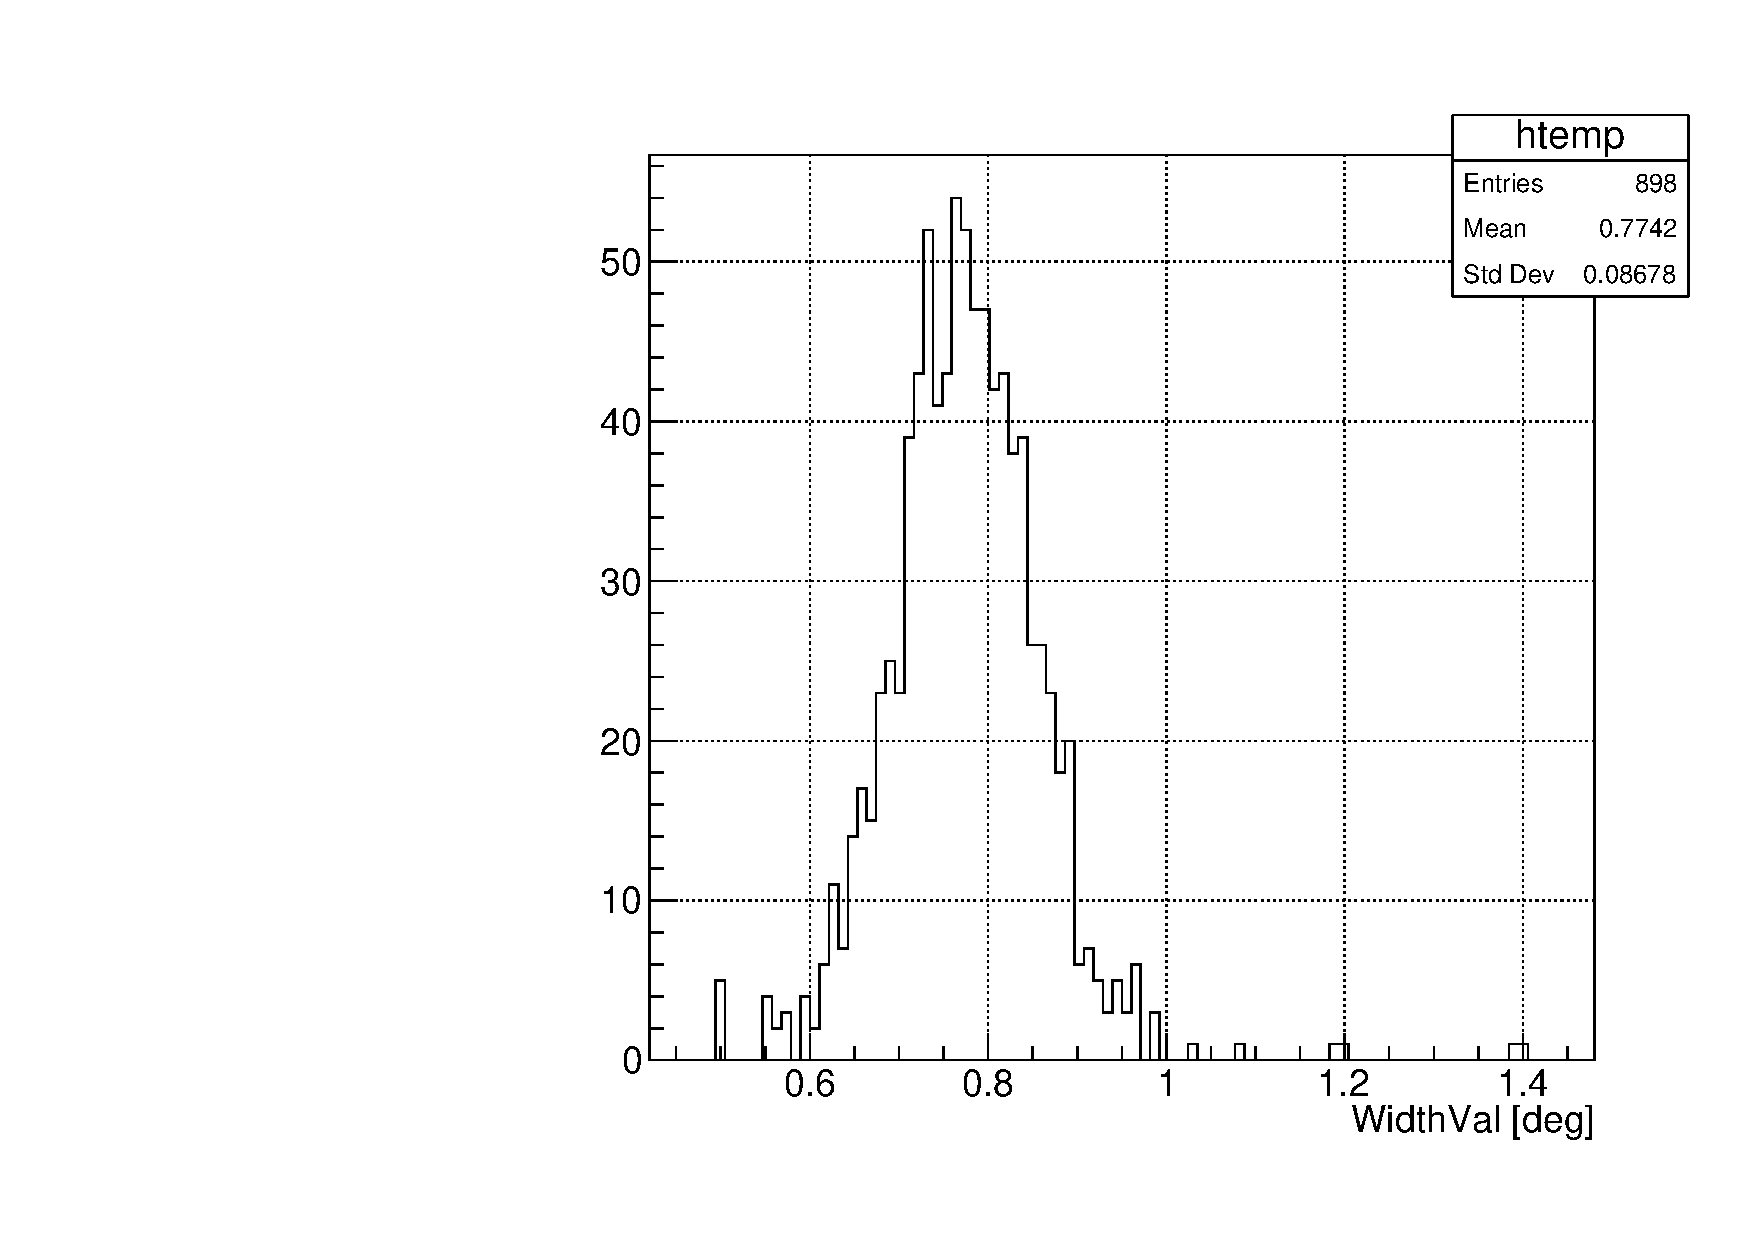
\includegraphics[width=.4\linewidth]{plots/2018/PhiWidthVal.pdf}
    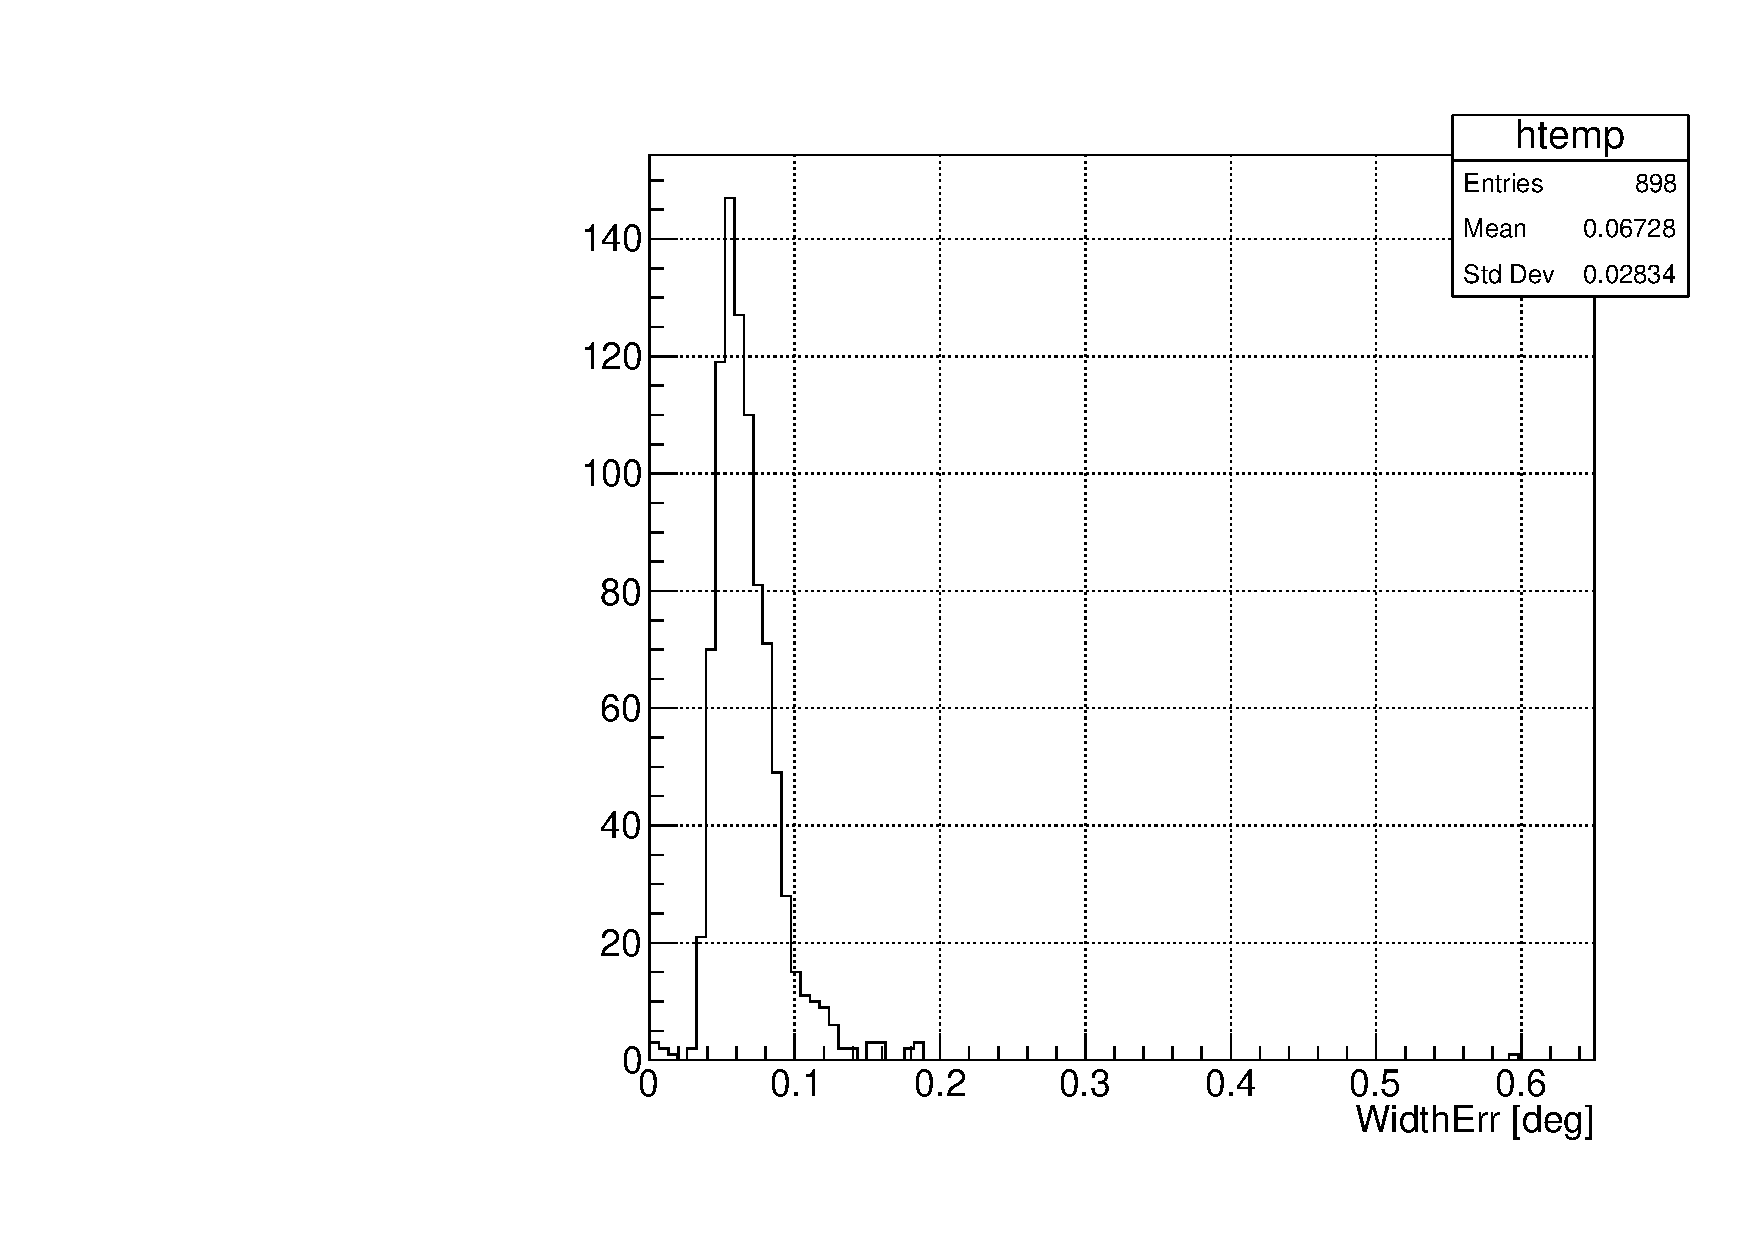
\includegraphics[width=.4\linewidth]{plots/2018/PhiWidthErr.pdf}\\
    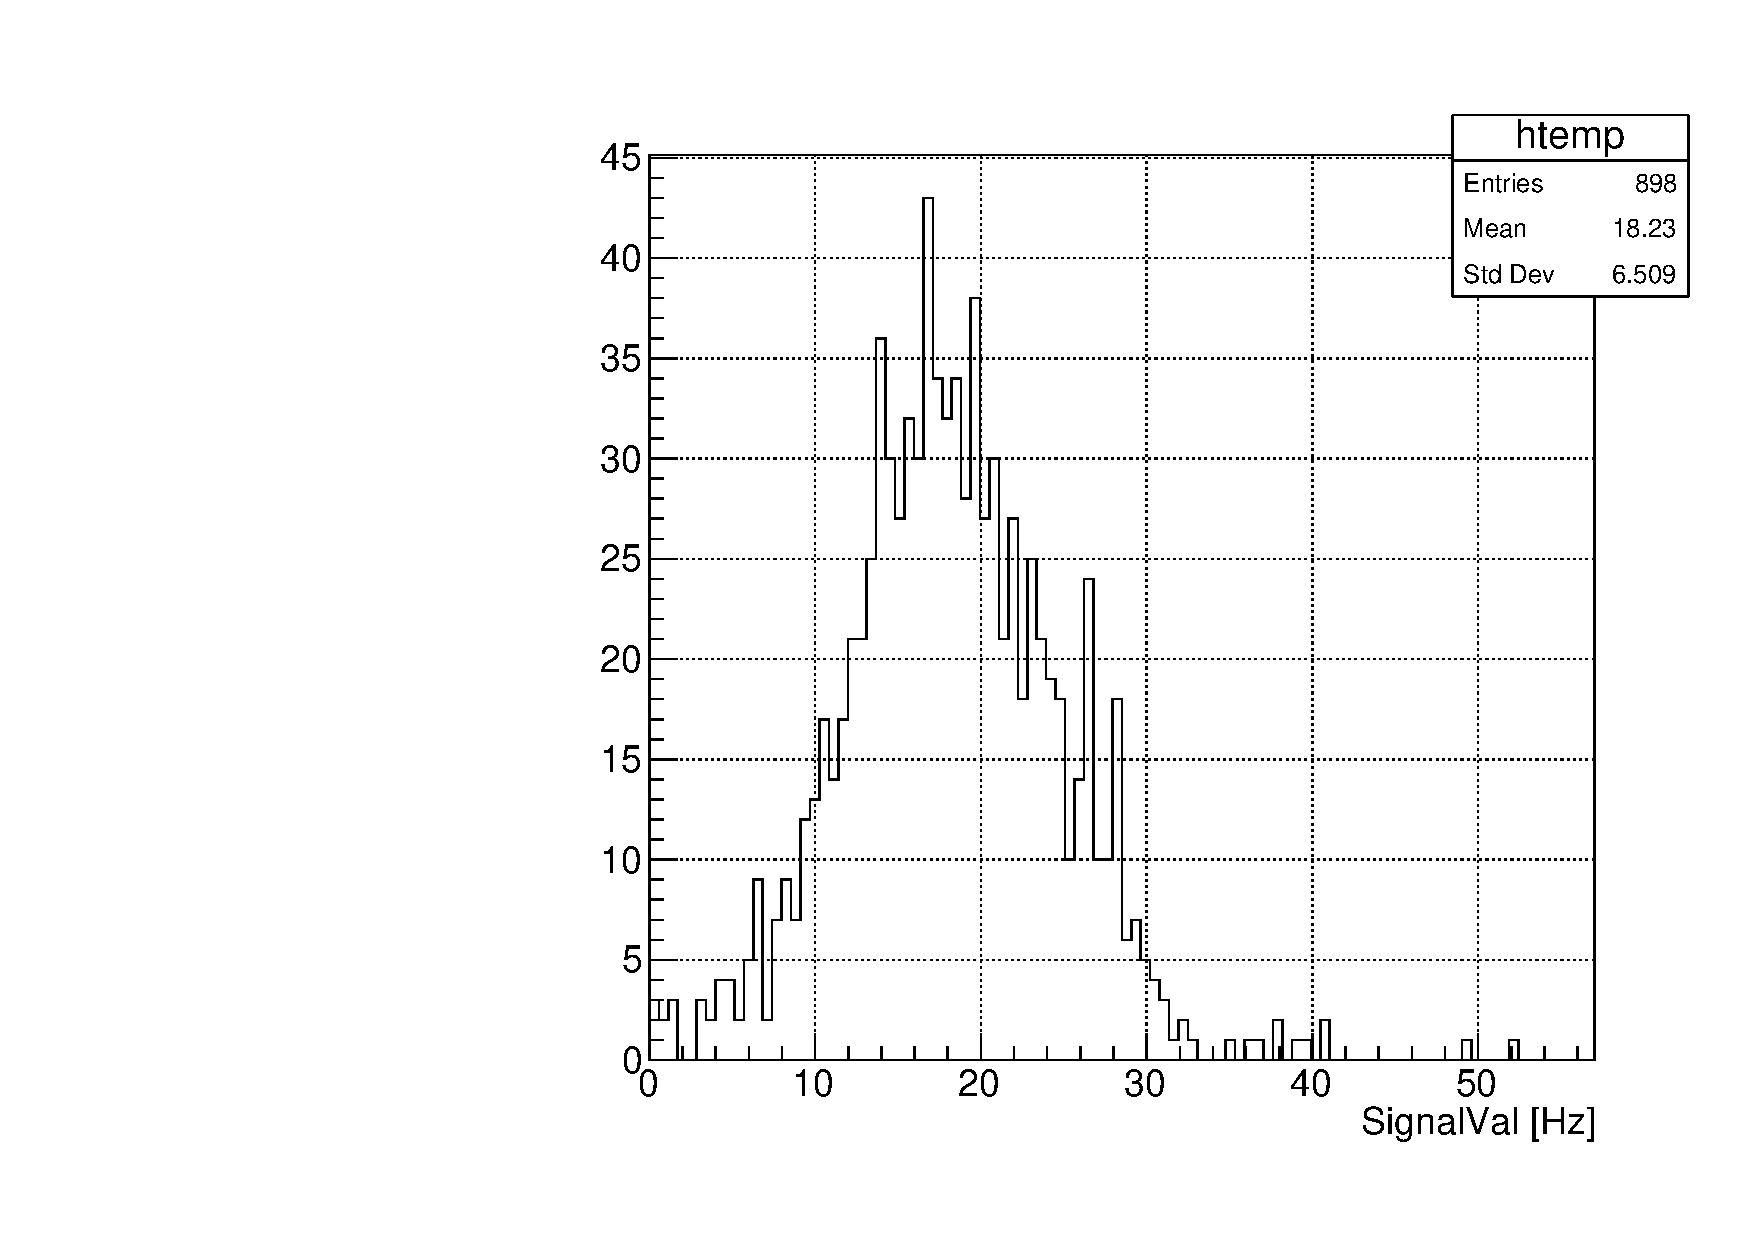
\includegraphics[width=.4\linewidth]{plots/2018/PhiSignalVal.pdf}
    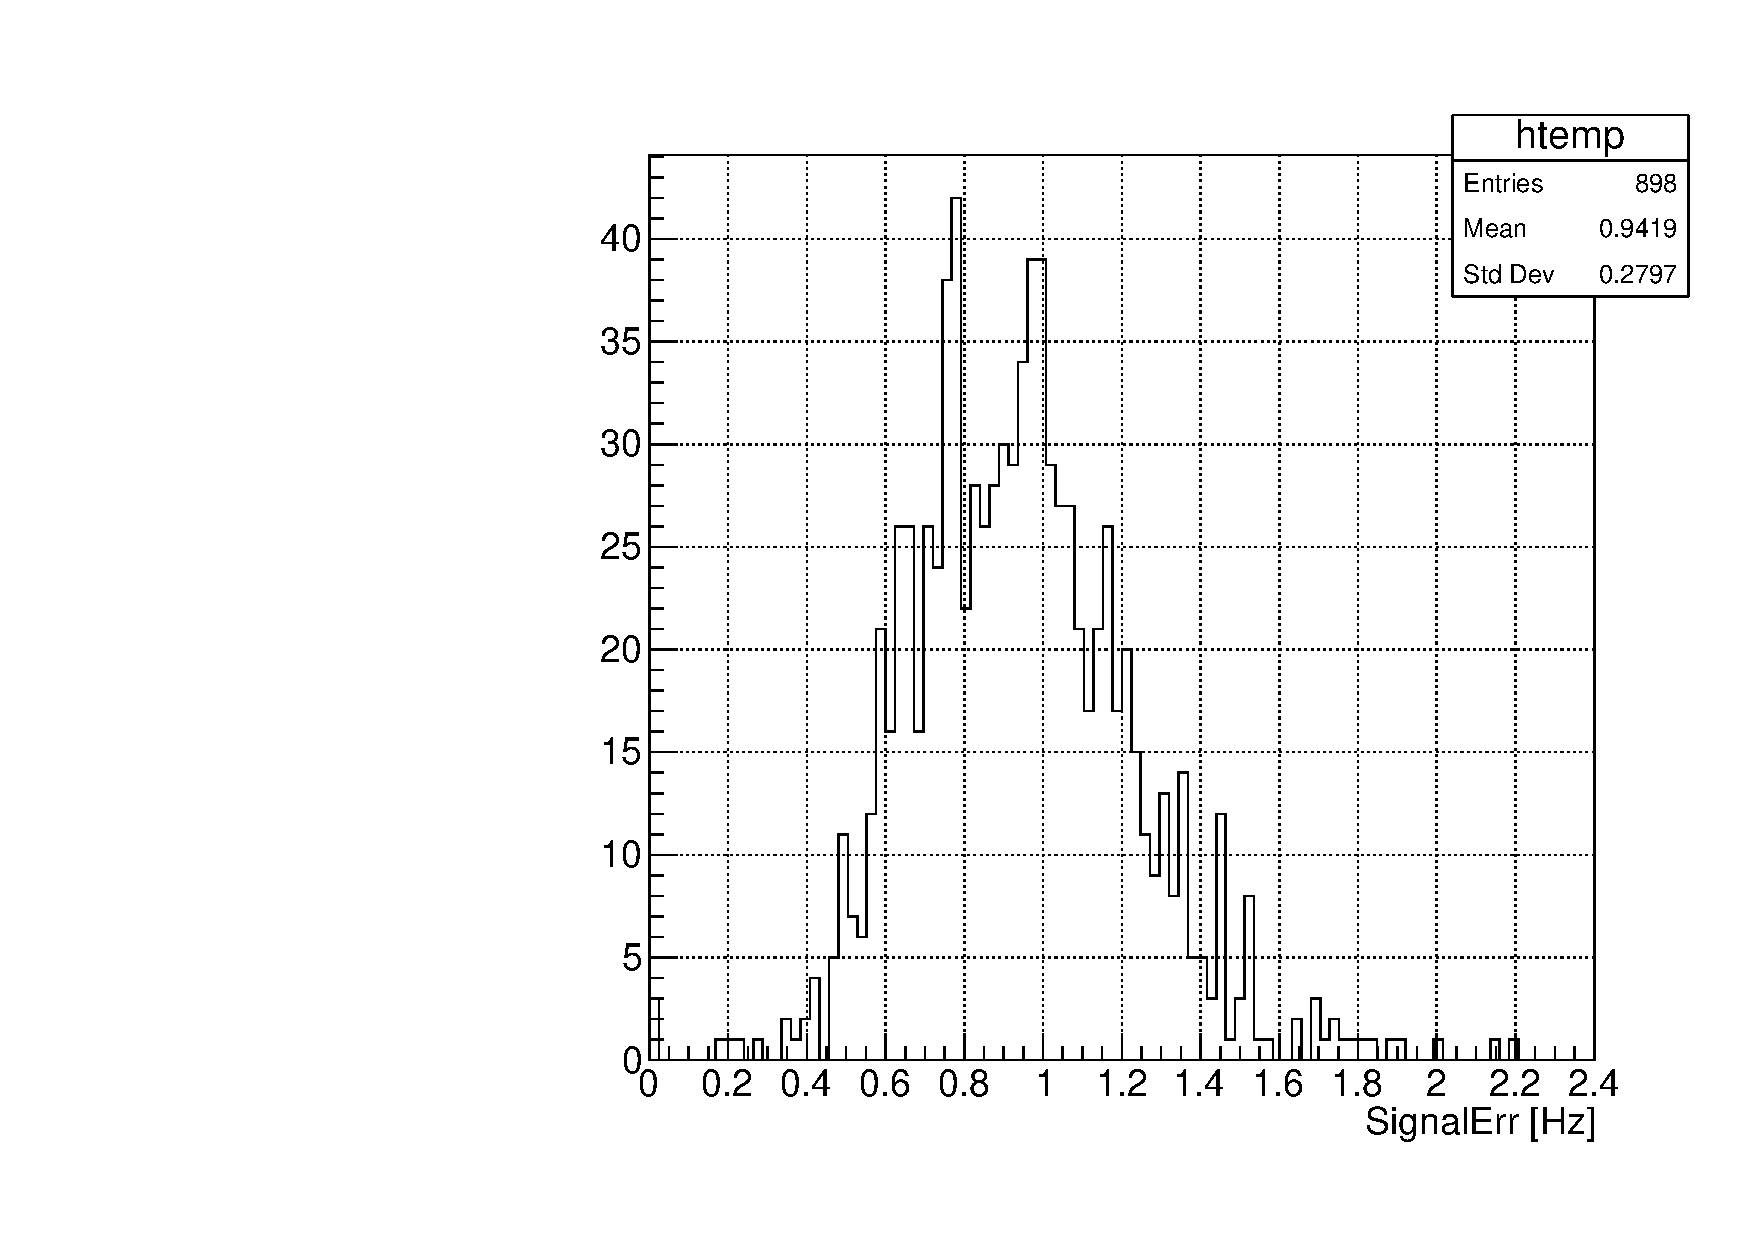
\includegraphics[width=.4\linewidth]{plots/2018/PhiSignalErr.pdf}\\
    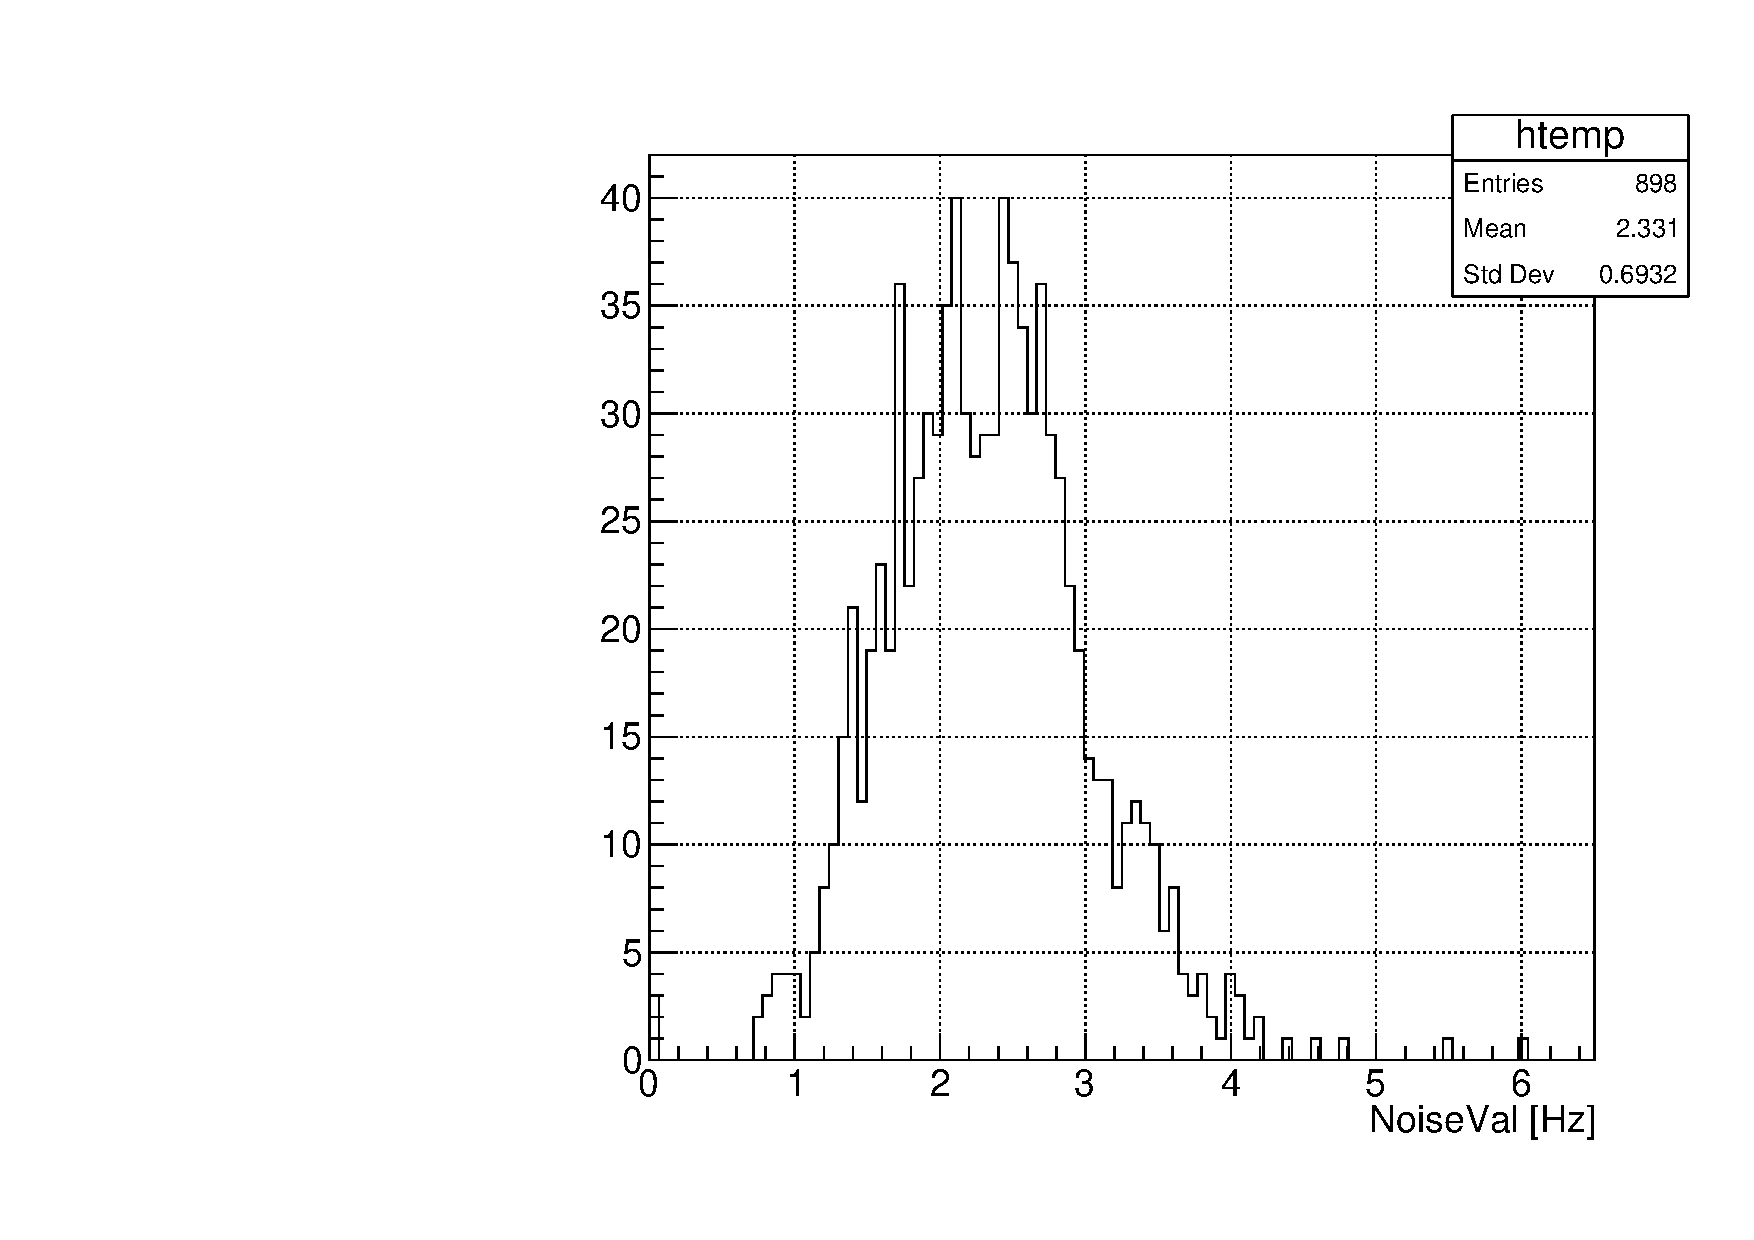
\includegraphics[width=.4\linewidth]{plots/2018/PhiNoiseVal.pdf}
    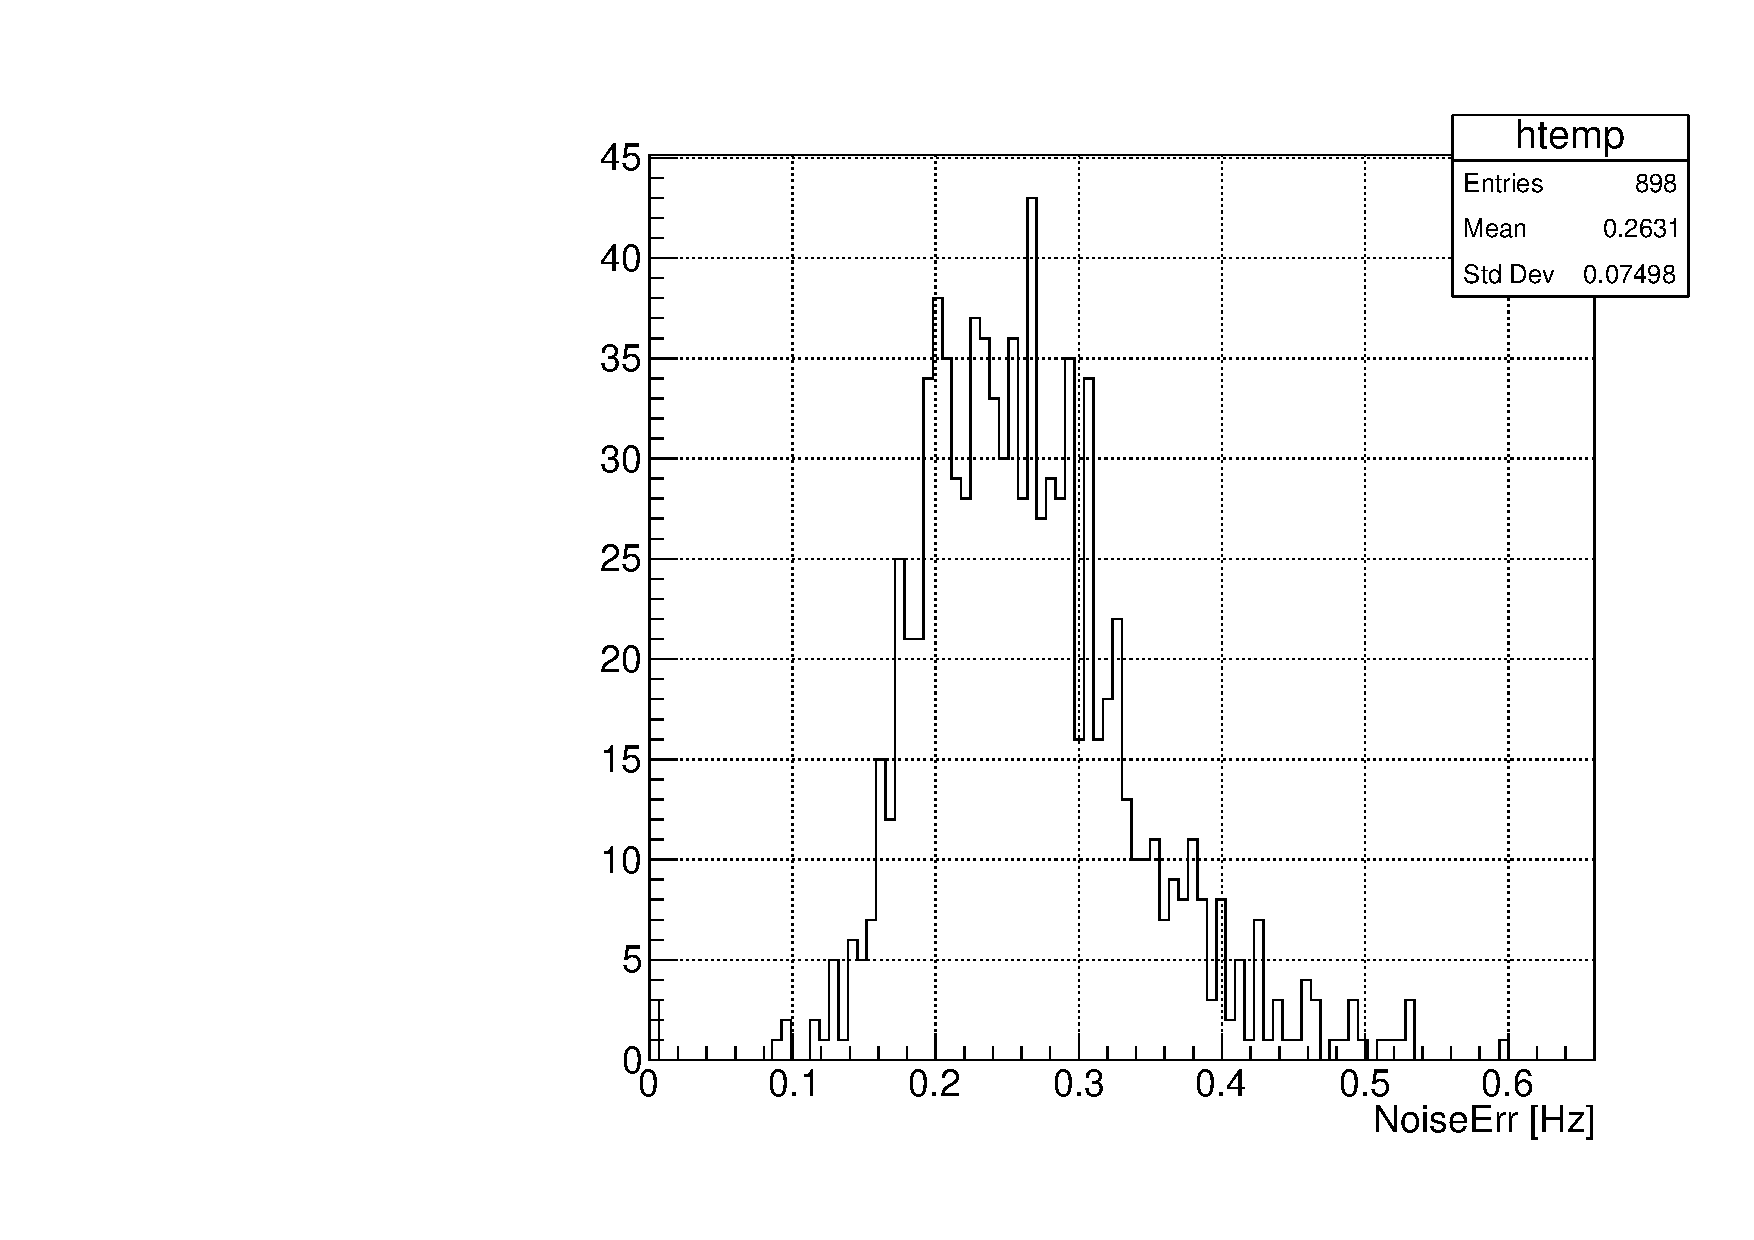
\includegraphics[width=.4\linewidth]{plots/2018/PhiNoiseErr.pdf}
    \caption{Fitted parameter values (left) and errors (right) for $\phi$ position fits.}
    \label{fig:zfitpars}
\end{figure}
